\documentclass[twoside]{book}

% Packages required by doxygen
\usepackage{fixltx2e}
\usepackage{calc}
\usepackage{doxygen}
\usepackage[export]{adjustbox} % also loads graphicx
\usepackage{graphicx}
\usepackage[utf8]{inputenc}
\usepackage{makeidx}
\usepackage{multicol}
\usepackage{multirow}
\PassOptionsToPackage{warn}{textcomp}
\usepackage{textcomp}
\usepackage[nointegrals]{wasysym}
\usepackage[table]{xcolor}

% Font selection
\usepackage[T1]{fontenc}
\usepackage[scaled=.90]{helvet}
\usepackage{courier}
\usepackage{amssymb}
\usepackage{sectsty}
\renewcommand{\familydefault}{\sfdefault}
\allsectionsfont{%
  \fontseries{bc}\selectfont%
  \color{darkgray}%
}
\renewcommand{\DoxyLabelFont}{%
  \fontseries{bc}\selectfont%
  \color{darkgray}%
}
\newcommand{\+}{\discretionary{\mbox{\scriptsize$\hookleftarrow$}}{}{}}

% Page & text layout
\usepackage{geometry}
\geometry{%
  a4paper,%
  top=2.5cm,%
  bottom=2.5cm,%
  left=2.5cm,%
  right=2.5cm%
}
\tolerance=750
\hfuzz=15pt
\hbadness=750
\setlength{\emergencystretch}{15pt}
\setlength{\parindent}{0cm}
\setlength{\parskip}{3ex plus 2ex minus 2ex}
\makeatletter
\renewcommand{\paragraph}{%
  \@startsection{paragraph}{4}{0ex}{-1.0ex}{1.0ex}{%
    \normalfont\normalsize\bfseries\SS@parafont%
  }%
}
\renewcommand{\subparagraph}{%
  \@startsection{subparagraph}{5}{0ex}{-1.0ex}{1.0ex}{%
    \normalfont\normalsize\bfseries\SS@subparafont%
  }%
}
\makeatother

% Headers & footers
\usepackage{fancyhdr}
\pagestyle{fancyplain}
\fancyhead[LE]{\fancyplain{}{\bfseries\thepage}}
\fancyhead[CE]{\fancyplain{}{}}
\fancyhead[RE]{\fancyplain{}{\bfseries\leftmark}}
\fancyhead[LO]{\fancyplain{}{\bfseries\rightmark}}
\fancyhead[CO]{\fancyplain{}{}}
\fancyhead[RO]{\fancyplain{}{\bfseries\thepage}}
\fancyfoot[LE]{\fancyplain{}{}}
\fancyfoot[CE]{\fancyplain{}{}}
\fancyfoot[RE]{\fancyplain{}{\bfseries\scriptsize Generated by Doxygen }}
\fancyfoot[LO]{\fancyplain{}{\bfseries\scriptsize Generated by Doxygen }}
\fancyfoot[CO]{\fancyplain{}{}}
\fancyfoot[RO]{\fancyplain{}{}}
\renewcommand{\footrulewidth}{0.4pt}
\renewcommand{\chaptermark}[1]{%
  \markboth{#1}{}%
}
\renewcommand{\sectionmark}[1]{%
  \markright{\thesection\ #1}%
}

% Indices & bibliography
\usepackage{natbib}
\usepackage[titles]{tocloft}
\setcounter{tocdepth}{3}
\setcounter{secnumdepth}{5}
\makeindex

% Hyperlinks (required, but should be loaded last)
\usepackage{ifpdf}
\ifpdf
  \usepackage[pdftex,pagebackref=true]{hyperref}
\else
  \usepackage[ps2pdf,pagebackref=true]{hyperref}
\fi
\hypersetup{%
  colorlinks=true,%
  linkcolor=blue,%
  citecolor=blue,%
  unicode%
}

% Custom commands
\newcommand{\clearemptydoublepage}{%
  \newpage{\pagestyle{empty}\cleardoublepage}%
}

\usepackage{caption}
\captionsetup{labelsep=space,justification=centering,font={bf},singlelinecheck=off,skip=4pt,position=top}

%===== C O N T E N T S =====

\begin{document}

% Titlepage & ToC
\hypersetup{pageanchor=false,
             bookmarksnumbered=true,
             pdfencoding=unicode
            }
\pagenumbering{alph}
\begin{titlepage}
\vspace*{7cm}
\begin{center}%
{\Large sledgehamr }\\
\vspace*{1cm}
{\large Generated by Doxygen 1.8.14}\\
\end{center}
\end{titlepage}
\clearemptydoublepage
\pagenumbering{roman}
\tableofcontents
\clearemptydoublepage
\pagenumbering{arabic}
\hypersetup{pageanchor=true}

%--- Begin generated contents ---
\chapter{Namespace Index}
\section{Namespace List}
Here is a list of all documented namespaces with brief descriptions\+:\begin{DoxyCompactList}
\item\contentsline{section}{\mbox{\hyperlink{namespacesledgehamr}{sledgehamr}} }{\pageref{namespacesledgehamr}}{}
\end{DoxyCompactList}

\chapter{Hierarchical Index}
\section{Class Hierarchy}
This inheritance list is sorted roughly, but not completely, alphabetically\+:\begin{DoxyCompactList}
\item Amr\+Core\begin{DoxyCompactList}
\item \contentsline{section}{sledgehamr\+:\+:Sledgehamr}{\pageref{classsledgehamr_1_1Sledgehamr}}{}
\end{DoxyCompactList}
\item \contentsline{section}{py\+Sledgehamr.\+Axion\+Strings.\+Axion\+Strings}{\pageref{classpySledgehamr_1_1AxionStrings_1_1AxionStrings}}{}
\item \contentsline{section}{sledgehamr\+:\+:Fill\+Level}{\pageref{classsledgehamr_1_1FillLevel}}{}
\item \contentsline{section}{sledgehamr\+:\+:Gravitational\+Waves}{\pageref{classsledgehamr_1_1GravitationalWaves}}{}
\item \contentsline{section}{sledgehamr\+:\+:I\+O\+Module}{\pageref{classsledgehamr_1_1IOModule}}{}
\item \contentsline{section}{sledgehamr\+:\+:Level\+Synchronizer}{\pageref{classsledgehamr_1_1LevelSynchronizer}}{}
\item Multi\+Fab\begin{DoxyCompactList}
\item \contentsline{section}{sledgehamr\+:\+:Level\+Data}{\pageref{classsledgehamr_1_1LevelData}}{}
\end{DoxyCompactList}
\item \contentsline{section}{sledgehamr\+:\+:Null\+Fill}{\pageref{structsledgehamr_1_1NullFill}}{}
\item \contentsline{section}{py\+Sledgehamr.\+Output.\+Output}{\pageref{classpySledgehamr_1_1Output_1_1Output}}{}
\item \contentsline{section}{sledgehamr\+:\+:Performance\+Monitor}{\pageref{classsledgehamr_1_1PerformanceMonitor}}{}
\item \contentsline{section}{sledgehamr\+:\+:Regrid\+Scheduler}{\pageref{classsledgehamr_1_1RegridScheduler}}{}
\item \contentsline{section}{sledgehamr\+:\+:Scalar\+Field}{\pageref{classsledgehamr_1_1ScalarField}}{}
\item \contentsline{section}{sledgehamr\+:\+:Scheduled\+Regrid}{\pageref{classsledgehamr_1_1ScheduledRegrid}}{}
\item \contentsline{section}{sledgehamr\+:\+:Sledgehamr\+Init}{\pageref{classsledgehamr_1_1SledgehamrInit}}{}
\item \contentsline{section}{sledgehamr\+:\+:Timer}{\pageref{classsledgehamr_1_1Timer}}{}
\item \contentsline{section}{sledgehamr\+:\+:Time\+Stepper}{\pageref{classsledgehamr_1_1TimeStepper}}{}
\end{DoxyCompactList}

\chapter{Class Index}
\section{Class List}
Here are the classes, structs, unions and interfaces with brief descriptions\+:\begin{DoxyCompactList}
\item\contentsline{section}{\mbox{\hyperlink{classpySledgehamr_1_1AxionStrings_1_1AxionStrings}{py\+Sledgehamr.\+Axion\+Strings.\+Axion\+Strings}} \\*Class that handles everything special for the Axion string project such as creating initial states and computing the string length and axion spectra }{\pageref{classpySledgehamr_1_1AxionStrings_1_1AxionStrings}}{}
\item\contentsline{section}{\mbox{\hyperlink{classsledgehamr_1_1FillLevel}{sledgehamr\+::\+Fill\+Level}} }{\pageref{classsledgehamr_1_1FillLevel}}{}
\item\contentsline{section}{\mbox{\hyperlink{classsledgehamr_1_1GravitationalWaves}{sledgehamr\+::\+Gravitational\+Waves}} }{\pageref{classsledgehamr_1_1GravitationalWaves}}{}
\item\contentsline{section}{\mbox{\hyperlink{classsledgehamr_1_1IOModule}{sledgehamr\+::\+I\+O\+Module}} \\*Class that handles all I/O operations besides parsing the inputs file }{\pageref{classsledgehamr_1_1IOModule}}{}
\item\contentsline{section}{\mbox{\hyperlink{classsledgehamr_1_1LevelData}{sledgehamr\+::\+Level\+Data}} \\*Class that holds the Multi\+Fab data while also keeping track of time and step numbers }{\pageref{classsledgehamr_1_1LevelData}}{}
\item\contentsline{section}{\mbox{\hyperlink{classsledgehamr_1_1LevelSynchronizer}{sledgehamr\+::\+Level\+Synchronizer}} \\*This class handles all operations between two levels such as averaging down, interpolation to fine, filling of ghost cells, etc. Class is friend of Sledge\+H\+A\+MR }{\pageref{classsledgehamr_1_1LevelSynchronizer}}{}
\item\contentsline{section}{\mbox{\hyperlink{structsledgehamr_1_1NullFill}{sledgehamr\+::\+Null\+Fill}} \\*Struct with overloaded operator to handle boundary conditions. Empty because we do not have boundary conditions beyond periodic }{\pageref{structsledgehamr_1_1NullFill}}{}
\item\contentsline{section}{\mbox{\hyperlink{classpySledgehamr_1_1Output_1_1Output}{py\+Sledgehamr.\+Output.\+Output}} \\*This class reads all Sledge\+H\+A\+MR output }{\pageref{classpySledgehamr_1_1Output_1_1Output}}{}
\item\contentsline{section}{\mbox{\hyperlink{classsledgehamr_1_1PerformanceMonitor}{sledgehamr\+::\+Performance\+Monitor}} }{\pageref{classsledgehamr_1_1PerformanceMonitor}}{}
\item\contentsline{section}{\mbox{\hyperlink{classsledgehamr_1_1RegridScheduler}{sledgehamr\+::\+Regrid\+Scheduler}} }{\pageref{classsledgehamr_1_1RegridScheduler}}{}
\item\contentsline{section}{\mbox{\hyperlink{classsledgehamr_1_1ScalarField}{sledgehamr\+::\+Scalar\+Field}} \\*Class to keep track of scalar fields }{\pageref{classsledgehamr_1_1ScalarField}}{}
\item\contentsline{section}{\mbox{\hyperlink{classsledgehamr_1_1ScheduledRegrid}{sledgehamr\+::\+Scheduled\+Regrid}} }{\pageref{classsledgehamr_1_1ScheduledRegrid}}{}
\item\contentsline{section}{\mbox{\hyperlink{classsledgehamr_1_1Sledgehamr}{sledgehamr\+::\+Sledgehamr}} \\*Base class for all derived projects. Combines all the ingredients to make this code work }{\pageref{classsledgehamr_1_1Sledgehamr}}{}
\item\contentsline{section}{\mbox{\hyperlink{classsledgehamr_1_1SledgehamrInit}{sledgehamr\+::\+Sledgehamr\+Init}} \\*Determines with project has been requested. Also feeds extra derived information to amrex\+::\+Amr\+Core }{\pageref{classsledgehamr_1_1SledgehamrInit}}{}
\item\contentsline{section}{\mbox{\hyperlink{classsledgehamr_1_1Timer}{sledgehamr\+::\+Timer}} }{\pageref{classsledgehamr_1_1Timer}}{}
\item\contentsline{section}{\mbox{\hyperlink{classsledgehamr_1_1TimeStepper}{sledgehamr\+::\+Time\+Stepper}} \\*Class that takes care of the sub-\/cycling in time algorithm as well as the scheduling regrids }{\pageref{classsledgehamr_1_1TimeStepper}}{}
\end{DoxyCompactList}

\chapter{Namespace Documentation}
\hypertarget{namespacesledgehamr}{}\section{sledgehamr Namespace Reference}
\label{namespacesledgehamr}\index{sledgehamr@{sledgehamr}}
\subsection*{Classes}
\begin{DoxyCompactItemize}
\item 
class \mbox{\hyperlink{classsledgehamr_1_1FillLevel}{Fill\+Level}}
\item 
class \mbox{\hyperlink{classsledgehamr_1_1GravitationalWaves}{Gravitational\+Waves}}
\item 
class \mbox{\hyperlink{classsledgehamr_1_1IOModule}{I\+O\+Module}}
\begin{DoxyCompactList}\small\item\em Class that handles all I/O operations besides parsing the inputs file. \end{DoxyCompactList}\item 
class \mbox{\hyperlink{classsledgehamr_1_1LevelData}{Level\+Data}}
\begin{DoxyCompactList}\small\item\em Class that holds the Multi\+Fab data while also keeping track of time and step numbers. \end{DoxyCompactList}\item 
class \mbox{\hyperlink{classsledgehamr_1_1LevelSynchronizer}{Level\+Synchronizer}}
\begin{DoxyCompactList}\small\item\em This class handles all operations between two levels such as averaging down, interpolation to fine, filling of ghost cells, etc. Class is friend of Sledge\+H\+A\+MR. \end{DoxyCompactList}\item 
struct \mbox{\hyperlink{structsledgehamr_1_1NullFill}{Null\+Fill}}
\begin{DoxyCompactList}\small\item\em Struct with overloaded operator to handle boundary conditions. Empty because we do not have boundary conditions beyond periodic. \end{DoxyCompactList}\item 
class \mbox{\hyperlink{classsledgehamr_1_1PerformanceMonitor}{Performance\+Monitor}}
\item 
class \mbox{\hyperlink{classsledgehamr_1_1RegridScheduler}{Regrid\+Scheduler}}
\item 
class \mbox{\hyperlink{classsledgehamr_1_1ScalarField}{Scalar\+Field}}
\begin{DoxyCompactList}\small\item\em Class to keep track of scalar fields. \end{DoxyCompactList}\item 
class \mbox{\hyperlink{classsledgehamr_1_1ScheduledRegrid}{Scheduled\+Regrid}}
\item 
class \mbox{\hyperlink{classsledgehamr_1_1Sledgehamr}{Sledgehamr}}
\begin{DoxyCompactList}\small\item\em Base class for all derived projects. Combines all the ingredients to make this code work. \end{DoxyCompactList}\item 
class \mbox{\hyperlink{classsledgehamr_1_1SledgehamrInit}{Sledgehamr\+Init}}
\begin{DoxyCompactList}\small\item\em Determines with project has been requested. Also feeds extra derived information to amrex\+::\+Amr\+Core. \end{DoxyCompactList}\item 
class \mbox{\hyperlink{classsledgehamr_1_1Timer}{Timer}}
\item 
class \mbox{\hyperlink{classsledgehamr_1_1TimeStepper}{Time\+Stepper}}
\begin{DoxyCompactList}\small\item\em Class that takes care of the sub-\/cycling in time algorithm as well as the scheduling regrids. \end{DoxyCompactList}\end{DoxyCompactItemize}


\subsection{Detailed Description}
Yes, I know this file is disgusting. This is what we get for not wanting everyone to write a bunch of complicated boilerplate every single time but also want to avoid all this function overhead for performance ... 
\chapter{Class Documentation}
\hypertarget{classpySledgehamr_1_1AxionStrings_1_1AxionStrings}{}\section{py\+Sledgehamr.\+Axion\+Strings.\+Axion\+Strings Class Reference}
\label{classpySledgehamr_1_1AxionStrings_1_1AxionStrings}\index{py\+Sledgehamr.\+Axion\+Strings.\+Axion\+Strings@{py\+Sledgehamr.\+Axion\+Strings.\+Axion\+Strings}}


Class that handles everything special for the Axion string project such as creating initial states and computing the string length and axion spectra.  


\subsection*{Public Member Functions}
\begin{DoxyCompactItemize}
\item 
def \mbox{\hyperlink{classpySledgehamr_1_1AxionStrings_1_1AxionStrings_a07c5c2f5cc07773e41091bf139771edd}{Create\+Initial\+State}} (self, L, N, k\+\_\+max, t\+\_\+start, output\+\_\+file, lambda\+\_\+param=1., sim\+\_\+output\+\_\+with\+\_\+box\+\_\+layout=\textquotesingle{}\textquotesingle{})
\begin{DoxyCompactList}\small\item\em Creates an initial state for Psi1, Psi2, Pi1, and Pi2. \end{DoxyCompactList}\item 
\mbox{\Hypertarget{classpySledgehamr_1_1AxionStrings_1_1AxionStrings_a0bb4272e44918593cb4c6057ed170c6e}\label{classpySledgehamr_1_1AxionStrings_1_1AxionStrings_a0bb4272e44918593cb4c6057ed170c6e}} 
def {\bfseries Get\+Xi} (self, output\+\_\+folder)
\item 
\mbox{\Hypertarget{classpySledgehamr_1_1AxionStrings_1_1AxionStrings_a48774f18d62004980be46e7de8e77be9}\label{classpySledgehamr_1_1AxionStrings_1_1AxionStrings_a48774f18d62004980be46e7de8e77be9}} 
def {\bfseries Plot\+Axion\+And\+Radial\+Mode\+Slice} (self, axion, radial\+\_\+mode, save\+\_\+name=\char`\"{}\char`\"{})
\end{DoxyCompactItemize}


\subsection{Detailed Description}
Class that handles everything special for the Axion string project such as creating initial states and computing the string length and axion spectra. 



\subsection{Member Function Documentation}
\mbox{\Hypertarget{classpySledgehamr_1_1AxionStrings_1_1AxionStrings_a07c5c2f5cc07773e41091bf139771edd}\label{classpySledgehamr_1_1AxionStrings_1_1AxionStrings_a07c5c2f5cc07773e41091bf139771edd}} 
\index{py\+Sledgehamr\+::\+Axion\+Strings\+::\+Axion\+Strings@{py\+Sledgehamr\+::\+Axion\+Strings\+::\+Axion\+Strings}!Create\+Initial\+State@{Create\+Initial\+State}}
\index{Create\+Initial\+State@{Create\+Initial\+State}!py\+Sledgehamr\+::\+Axion\+Strings\+::\+Axion\+Strings@{py\+Sledgehamr\+::\+Axion\+Strings\+::\+Axion\+Strings}}
\subsubsection{\texorpdfstring{Create\+Initial\+State()}{CreateInitialState()}}
{\footnotesize\ttfamily def py\+Sledgehamr.\+Axion\+Strings.\+Axion\+Strings.\+Create\+Initial\+State (\begin{DoxyParamCaption}\item[{}]{self,  }\item[{}]{L,  }\item[{}]{N,  }\item[{}]{k\+\_\+max,  }\item[{}]{t\+\_\+start,  }\item[{}]{output\+\_\+file,  }\item[{}]{lambda\+\_\+param = {\ttfamily 1.},  }\item[{}]{sim\+\_\+output\+\_\+with\+\_\+box\+\_\+layout = {\ttfamily \textquotesingle{}\textquotesingle{}} }\end{DoxyParamCaption})}



Creates an initial state for Psi1, Psi2, Pi1, and Pi2. 


\begin{DoxyParams}{Parameters}
{\em L} & Box length in units of 1/(a\+\_\+1 H\+\_\+1). \\
\hline
{\em N} & Number of coarse level grid sites. \\
\hline
{\em k\+\_\+max} & Maximum wave number to be included. \\
\hline
{\em output\+\_\+file} & Name of output file (must include prefix). \\
\hline
{\em lambda\+\_\+param} & Coupling parameter lambda. \\
\hline
\end{DoxyParams}


The documentation for this class was generated from the following file\+:\begin{DoxyCompactItemize}
\item 
/global/cfs/cdirs/m3166/buschman/sledgehamr/py\+Sledgehamr/Axion\+Strings.\+py\end{DoxyCompactItemize}

\hypertarget{classsledgehamr_1_1FillLevel}{}\section{sledgehamr\+:\+:Fill\+Level Class Reference}
\label{classsledgehamr_1_1FillLevel}\index{sledgehamr\+::\+Fill\+Level@{sledgehamr\+::\+Fill\+Level}}
\subsection*{Public Member Functions}
\begin{DoxyCompactItemize}
\item 
\mbox{\Hypertarget{classsledgehamr_1_1FillLevel_a15e50c8e83fb02a3e7cfadf75d798c39}\label{classsledgehamr_1_1FillLevel_a15e50c8e83fb02a3e7cfadf75d798c39}} 
{\bfseries Fill\+Level} (\mbox{\hyperlink{classsledgehamr_1_1Sledgehamr}{Sledgehamr}} $\ast$owner, int level)
\item 
\mbox{\Hypertarget{classsledgehamr_1_1FillLevel_a32272a06c4a4238f47b008220a449f87}\label{classsledgehamr_1_1FillLevel_a32272a06c4a4238f47b008220a449f87}} 
void {\bfseries From\+Initial\+State\+File} ()
\item 
\mbox{\Hypertarget{classsledgehamr_1_1FillLevel_ad7a535ae81fe6b4b3160fabee939294e}\label{classsledgehamr_1_1FillLevel_ad7a535ae81fe6b4b3160fabee939294e}} 
void {\bfseries From\+Checkpoint\+File} (std\+::string folder)
\item 
\mbox{\Hypertarget{classsledgehamr_1_1FillLevel_a204b7748191f00332384512697e2bc83}\label{classsledgehamr_1_1FillLevel_a204b7748191f00332384512697e2bc83}} 
void {\bfseries From\+Hdf5\+File} (std\+::string initial\+\_\+state\+\_\+file)
\item 
\mbox{\Hypertarget{classsledgehamr_1_1FillLevel_a47fcd3db3a286f70836366d0c1bb0274}\label{classsledgehamr_1_1FillLevel_a47fcd3db3a286f70836366d0c1bb0274}} 
void {\bfseries From\+Array} (const int comp, double $\ast$data, const long long dimN)
\item 
\mbox{\Hypertarget{classsledgehamr_1_1FillLevel_a422d6c8e962409de45ace3bfb3b41b7d}\label{classsledgehamr_1_1FillLevel_a422d6c8e962409de45ace3bfb3b41b7d}} 
void {\bfseries From\+Array\+Chunks} (const int comp, double $\ast$data)
\item 
\mbox{\Hypertarget{classsledgehamr_1_1FillLevel_a0cae844e7fe47a7bef70925b34ee436e}\label{classsledgehamr_1_1FillLevel_a0cae844e7fe47a7bef70925b34ee436e}} 
void {\bfseries From\+Const} (const int comp, const double c)
\end{DoxyCompactItemize}


The documentation for this class was generated from the following files\+:\begin{DoxyCompactItemize}
\item 
/global/cfs/cdirs/m3166/buschman/sledgehamr/source/fill\+\_\+level.\+h\item 
/global/cfs/cdirs/m3166/buschman/sledgehamr/source/fill\+\_\+level.\+cpp\end{DoxyCompactItemize}

\hypertarget{classsledgehamr_1_1GravitationalWaves}{}\section{sledgehamr\+:\+:Gravitational\+Waves Class Reference}
\label{classsledgehamr_1_1GravitationalWaves}\index{sledgehamr\+::\+Gravitational\+Waves@{sledgehamr\+::\+Gravitational\+Waves}}
\subsection*{Public Member Functions}
\begin{DoxyCompactItemize}
\item 
\mbox{\Hypertarget{classsledgehamr_1_1GravitationalWaves_a2d9489551b81e733bb1685023a3945b0}\label{classsledgehamr_1_1GravitationalWaves_a2d9489551b81e733bb1685023a3945b0}} 
{\bfseries Gravitational\+Waves} (\mbox{\hyperlink{classsledgehamr_1_1Sledgehamr}{Sledgehamr}} $\ast$owner)
\item 
\mbox{\Hypertarget{classsledgehamr_1_1GravitationalWaves_aa00cb3f7c6993a6bb7eb6d5475a6cfa0}\label{classsledgehamr_1_1GravitationalWaves_aa00cb3f7c6993a6bb7eb6d5475a6cfa0}} 
void {\bfseries Compute\+Spectrum} (hid\+\_\+t file\+\_\+id)
\end{DoxyCompactItemize}


The documentation for this class was generated from the following files\+:\begin{DoxyCompactItemize}
\item 
/global/cfs/cdirs/m3166/buschman/sledgehamr/source/gravitational\+\_\+waves.\+h\item 
/global/cfs/cdirs/m3166/buschman/sledgehamr/source/gravitational\+\_\+waves.\+cpp\end{DoxyCompactItemize}

\hypertarget{classsledgehamr_1_1IOModule}{}\section{sledgehamr\+:\+:I\+O\+Module Class Reference}
\label{classsledgehamr_1_1IOModule}\index{sledgehamr\+::\+I\+O\+Module@{sledgehamr\+::\+I\+O\+Module}}


Class that handles all I/O operations besides parsing the inputs file.  




{\ttfamily \#include $<$io\+\_\+module.\+h$>$}

\subsection*{Public Member Functions}
\begin{DoxyCompactItemize}
\item 
\mbox{\Hypertarget{classsledgehamr_1_1IOModule_aad737766170b477c2de5a30559798c07}\label{classsledgehamr_1_1IOModule_aad737766170b477c2de5a30559798c07}} 
{\bfseries I\+O\+Module} (\mbox{\hyperlink{classsledgehamr_1_1Sledgehamr}{Sledgehamr}} $\ast$owner)
\item 
\mbox{\Hypertarget{classsledgehamr_1_1IOModule_a00c504dbc9915e3fd10a0983cad67c5d}\label{classsledgehamr_1_1IOModule_a00c504dbc9915e3fd10a0983cad67c5d}} 
void \mbox{\hyperlink{classsledgehamr_1_1IOModule_a00c504dbc9915e3fd10a0983cad67c5d}{Write}} (bool force=false)
\begin{DoxyCompactList}\small\item\em Writes output if requested. \end{DoxyCompactList}\item 
\mbox{\Hypertarget{classsledgehamr_1_1IOModule_a6d40375399219df406fce38a63ce1ffb}\label{classsledgehamr_1_1IOModule_a6d40375399219df406fce38a63ce1ffb}} 
void {\bfseries Restart\+Sim} ()
\item 
\mbox{\Hypertarget{classsledgehamr_1_1IOModule_a716cbe1da6249ecaaa4023d70ce2f2cc}\label{classsledgehamr_1_1IOModule_a716cbe1da6249ecaaa4023d70ce2f2cc}} 
void {\bfseries Update\+Output\+Modules} ()
\item 
\mbox{\Hypertarget{classsledgehamr_1_1IOModule_a2d235a92fd8afd2e35586b2c5da6e72f}\label{classsledgehamr_1_1IOModule_a2d235a92fd8afd2e35586b2c5da6e72f}} 
void {\bfseries Write\+Box\+Array} (amrex\+::\+Box\+Array \&ba)
\end{DoxyCompactItemize}
\subsection*{Public Attributes}
\begin{DoxyCompactItemize}
\item 
\mbox{\Hypertarget{classsledgehamr_1_1IOModule_acf047b35679a313d50a8ca42be6c8956}\label{classsledgehamr_1_1IOModule_acf047b35679a313d50a8ca42be6c8956}} 
std\+::vector$<$ Projection $>$ \mbox{\hyperlink{classsledgehamr_1_1IOModule_acf047b35679a313d50a8ca42be6c8956}{projections}}
\begin{DoxyCompactList}\small\item\em Vectors containing instructions for projections and spectra. \end{DoxyCompactList}\item 
\mbox{\Hypertarget{classsledgehamr_1_1IOModule_a0d5e66413be2b95f3873eaa3fd55f8b9}\label{classsledgehamr_1_1IOModule_a0d5e66413be2b95f3873eaa3fd55f8b9}} 
std\+::vector$<$ Spectrum $>$ {\bfseries spectra}
\item 
\mbox{\Hypertarget{classsledgehamr_1_1IOModule_aa6af01cdd296efb0893eca1ef85bfbd0}\label{classsledgehamr_1_1IOModule_aa6af01cdd296efb0893eca1ef85bfbd0}} 
int \mbox{\hyperlink{classsledgehamr_1_1IOModule_aa6af01cdd296efb0893eca1ef85bfbd0}{idx\+\_\+slices}} = -\/1
\begin{DoxyCompactList}\small\item\em Easy access pointers for user-\/modifications. \end{DoxyCompactList}\item 
\mbox{\Hypertarget{classsledgehamr_1_1IOModule_a99784bd378acf2b2efabb7beb4315dbb}\label{classsledgehamr_1_1IOModule_a99784bd378acf2b2efabb7beb4315dbb}} 
int {\bfseries idx\+\_\+coarse\+\_\+box} = -\/1
\item 
\mbox{\Hypertarget{classsledgehamr_1_1IOModule_a6551a072168dbcdd788f892e27530173}\label{classsledgehamr_1_1IOModule_a6551a072168dbcdd788f892e27530173}} 
int {\bfseries idx\+\_\+full\+\_\+box} = -\/1
\item 
\mbox{\Hypertarget{classsledgehamr_1_1IOModule_a3c61a64fa45ddd8eced004a242db0e85}\label{classsledgehamr_1_1IOModule_a3c61a64fa45ddd8eced004a242db0e85}} 
int {\bfseries idx\+\_\+slices\+\_\+truncation\+\_\+error} = -\/1
\item 
\mbox{\Hypertarget{classsledgehamr_1_1IOModule_aace81c8a6d11eed4316b8021820dc39f}\label{classsledgehamr_1_1IOModule_aace81c8a6d11eed4316b8021820dc39f}} 
int {\bfseries idx\+\_\+coarse\+\_\+box\+\_\+truncation\+\_\+error} = -\/1
\item 
\mbox{\Hypertarget{classsledgehamr_1_1IOModule_a5ebafa73fe91df300dc49ff70b4a5649}\label{classsledgehamr_1_1IOModule_a5ebafa73fe91df300dc49ff70b4a5649}} 
int {\bfseries idx\+\_\+full\+\_\+box\+\_\+truncation\+\_\+error} = -\/1
\item 
\mbox{\Hypertarget{classsledgehamr_1_1IOModule_a6cfb269f85360b95e327cac02047e0fb}\label{classsledgehamr_1_1IOModule_a6cfb269f85360b95e327cac02047e0fb}} 
int {\bfseries idx\+\_\+projections} = -\/1
\item 
\mbox{\Hypertarget{classsledgehamr_1_1IOModule_a42ffd4132329490dc08f270952276a30}\label{classsledgehamr_1_1IOModule_a42ffd4132329490dc08f270952276a30}} 
int {\bfseries idx\+\_\+spectra} = -\/1
\item 
\mbox{\Hypertarget{classsledgehamr_1_1IOModule_a1dd7a15ede103d89d189120ac9a14dbd}\label{classsledgehamr_1_1IOModule_a1dd7a15ede103d89d189120ac9a14dbd}} 
int {\bfseries idx\+\_\+gw\+\_\+spectra} = -\/1
\item 
\mbox{\Hypertarget{classsledgehamr_1_1IOModule_a0b9a5b302433e479e6e6bcbb41739321}\label{classsledgehamr_1_1IOModule_a0b9a5b302433e479e6e6bcbb41739321}} 
int {\bfseries idx\+\_\+performance\+\_\+monitor} = -\/1
\item 
\mbox{\Hypertarget{classsledgehamr_1_1IOModule_af5434bf69e451f69064379b33a355634}\label{classsledgehamr_1_1IOModule_af5434bf69e451f69064379b33a355634}} 
int {\bfseries idx\+\_\+amrex\+\_\+plotfile} = -\/1
\item 
\mbox{\Hypertarget{classsledgehamr_1_1IOModule_adfb278d2d5b82d812b72d0cd6988b186}\label{classsledgehamr_1_1IOModule_adfb278d2d5b82d812b72d0cd6988b186}} 
int {\bfseries idx\+\_\+checkpoints} = -\/1
\item 
\mbox{\Hypertarget{classsledgehamr_1_1IOModule_ab093c90582020e1f9b7d8af3814e833a}\label{classsledgehamr_1_1IOModule_ab093c90582020e1f9b7d8af3814e833a}} 
std\+::vector$<$ Output\+Module $>$ \mbox{\hyperlink{classsledgehamr_1_1IOModule_ab093c90582020e1f9b7d8af3814e833a}{output}}
\begin{DoxyCompactList}\small\item\em Vector of output modules. \end{DoxyCompactList}\item 
\mbox{\Hypertarget{classsledgehamr_1_1IOModule_a411357720a9bfbb0f5dc6548090814dc}\label{classsledgehamr_1_1IOModule_a411357720a9bfbb0f5dc6548090814dc}} 
std\+::string {\bfseries output\+\_\+folder}
\item 
\mbox{\Hypertarget{classsledgehamr_1_1IOModule_af7545db0fa7ab4c5f6ffaaefcab579d2}\label{classsledgehamr_1_1IOModule_af7545db0fa7ab4c5f6ffaaefcab579d2}} 
std\+::string {\bfseries alternative\+\_\+output\+\_\+folder} = \char`\"{}\char`\"{}
\item 
\mbox{\Hypertarget{classsledgehamr_1_1IOModule_a9d75926888e4337742708c73db652bbb}\label{classsledgehamr_1_1IOModule_a9d75926888e4337742708c73db652bbb}} 
std\+::string {\bfseries old\+\_\+checkpoint} = \char`\"{}\char`\"{}
\end{DoxyCompactItemize}


\subsection{Detailed Description}
Class that handles all I/O operations besides parsing the inputs file. 

The documentation for this class was generated from the following files\+:\begin{DoxyCompactItemize}
\item 
/global/cfs/cdirs/m3166/buschman/sledgehamr/source/io\+\_\+module.\+h\item 
/global/cfs/cdirs/m3166/buschman/sledgehamr/source/io\+\_\+module.\+cpp\end{DoxyCompactItemize}

\hypertarget{classsledgehamr_1_1LevelData}{}\section{sledgehamr\+:\+:Level\+Data Class Reference}
\label{classsledgehamr_1_1LevelData}\index{sledgehamr\+::\+Level\+Data@{sledgehamr\+::\+Level\+Data}}


Class that holds the Multi\+Fab data while also keeping track of time and step numbers.  




{\ttfamily \#include $<$level\+\_\+data.\+h$>$}

Inheritance diagram for sledgehamr\+:\+:Level\+Data\+:\begin{figure}[H]
\begin{center}
\leavevmode
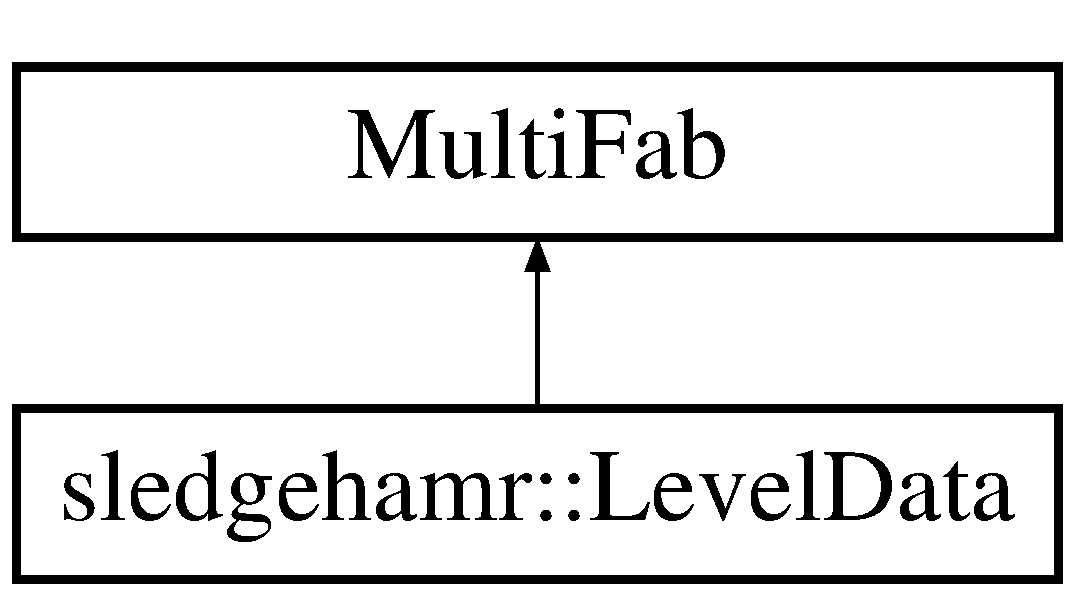
\includegraphics[height=2.000000cm]{classsledgehamr_1_1LevelData}
\end{center}
\end{figure}
\subsection*{Public Member Functions}
\begin{DoxyCompactItemize}
\item 
\mbox{\hyperlink{classsledgehamr_1_1LevelData_aa3e83b8e4d23e14648c511f80b6bfd39}{Level\+Data}} (amrex\+::\+Box\+Array ba, amrex\+::\+Distribution\+Mapping dm, int ncomp, int nghost, double time=0)
\begin{DoxyCompactList}\small\item\em Construct data using the given grid layout. \end{DoxyCompactList}\item 
void \mbox{\hyperlink{classsledgehamr_1_1LevelData_a5acdbd9ec718975bbf6c8c41f7a73b1a}{define}} (amrex\+::\+Box\+Array ba, amrex\+::\+Distribution\+Mapping dm, int ncomp, int nghost, double time)
\begin{DoxyCompactList}\small\item\em Overload amrex\+::\+Multi\+Fab\+::define function to include time. \end{DoxyCompactList}\end{DoxyCompactItemize}
\subsection*{Static Public Member Functions}
\begin{DoxyCompactItemize}
\item 
static amrex\+::\+Vector$<$ double $>$ \mbox{\hyperlink{classsledgehamr_1_1LevelData_a852bf27c741978378a87ce043cce3b24}{get\+Times}} (std\+::vector$<$ amrex\+::\+Multi\+Fab $\ast$$>$ \&mfs)
\begin{DoxyCompactList}\small\item\em Static method that returns vector of times from a given \mbox{\hyperlink{classsledgehamr_1_1LevelData}{Level\+Data}} vector. \end{DoxyCompactList}\end{DoxyCompactItemize}
\subsection*{Public Attributes}
\begin{DoxyCompactItemize}
\item 
\mbox{\Hypertarget{classsledgehamr_1_1LevelData_a9bc416cbd6054f0adb499ffd64144860}\label{classsledgehamr_1_1LevelData_a9bc416cbd6054f0adb499ffd64144860}} 
double \mbox{\hyperlink{classsledgehamr_1_1LevelData_a9bc416cbd6054f0adb499ffd64144860}{t}} = 0.
\begin{DoxyCompactList}\small\item\em Time corresponding to amrex\+::\+Multi\+Fab data. \end{DoxyCompactList}\item 
\mbox{\Hypertarget{classsledgehamr_1_1LevelData_a1fc20b81bee0349d0cc24a8407a42e3a}\label{classsledgehamr_1_1LevelData_a1fc20b81bee0349d0cc24a8407a42e3a}} 
int \mbox{\hyperlink{classsledgehamr_1_1LevelData_a1fc20b81bee0349d0cc24a8407a42e3a}{istep}} = 0
\begin{DoxyCompactList}\small\item\em How often this level has been advanced. \end{DoxyCompactList}\item 
\mbox{\Hypertarget{classsledgehamr_1_1LevelData_af4bc919d70ab9353c53c8e70e795777d}\label{classsledgehamr_1_1LevelData_af4bc919d70ab9353c53c8e70e795777d}} 
bool \mbox{\hyperlink{classsledgehamr_1_1LevelData_af4bc919d70ab9353c53c8e70e795777d}{contains\+\_\+truncation\+\_\+errors}} = false
\begin{DoxyCompactList}\small\item\em Flag as to whether the Mutli\+Fab has truncation errors encoded into it. \end{DoxyCompactList}\end{DoxyCompactItemize}


\subsection{Detailed Description}
Class that holds the Multi\+Fab data while also keeping track of time and step numbers. 

\subsection{Constructor \& Destructor Documentation}
\mbox{\Hypertarget{classsledgehamr_1_1LevelData_aa3e83b8e4d23e14648c511f80b6bfd39}\label{classsledgehamr_1_1LevelData_aa3e83b8e4d23e14648c511f80b6bfd39}} 
\index{sledgehamr\+::\+Level\+Data@{sledgehamr\+::\+Level\+Data}!Level\+Data@{Level\+Data}}
\index{Level\+Data@{Level\+Data}!sledgehamr\+::\+Level\+Data@{sledgehamr\+::\+Level\+Data}}
\subsubsection{\texorpdfstring{Level\+Data()}{LevelData()}}
{\footnotesize\ttfamily sledgehamr\+::\+Level\+Data\+::\+Level\+Data (\begin{DoxyParamCaption}\item[{amrex\+::\+Box\+Array}]{ba,  }\item[{amrex\+::\+Distribution\+Mapping}]{dm,  }\item[{int}]{ncomp,  }\item[{int}]{nghost,  }\item[{double}]{time = {\ttfamily 0} }\end{DoxyParamCaption})\hspace{0.3cm}{\ttfamily [inline]}}



Construct data using the given grid layout. 


\begin{DoxyParams}{Parameters}
{\em ba} & Box\+Array. \\
\hline
{\em dm} & Distribution\+Mapping. \\
\hline
{\em ncomp} & Total number of scalar fields components. \\
\hline
{\em nghost} & Number of ghost cells. \\
\hline
{\em time} & Time. \\
\hline
\end{DoxyParams}


\subsection{Member Function Documentation}
\mbox{\Hypertarget{classsledgehamr_1_1LevelData_a5acdbd9ec718975bbf6c8c41f7a73b1a}\label{classsledgehamr_1_1LevelData_a5acdbd9ec718975bbf6c8c41f7a73b1a}} 
\index{sledgehamr\+::\+Level\+Data@{sledgehamr\+::\+Level\+Data}!define@{define}}
\index{define@{define}!sledgehamr\+::\+Level\+Data@{sledgehamr\+::\+Level\+Data}}
\subsubsection{\texorpdfstring{define()}{define()}}
{\footnotesize\ttfamily void sledgehamr\+::\+Level\+Data\+::define (\begin{DoxyParamCaption}\item[{amrex\+::\+Box\+Array}]{ba,  }\item[{amrex\+::\+Distribution\+Mapping}]{dm,  }\item[{int}]{ncomp,  }\item[{int}]{nghost,  }\item[{double}]{time }\end{DoxyParamCaption})\hspace{0.3cm}{\ttfamily [inline]}}



Overload amrex\+::\+Multi\+Fab\+::define function to include time. 


\begin{DoxyParams}{Parameters}
{\em ba} & Box\+Array. \\
\hline
{\em dm} & Distribution\+Mapping. \\
\hline
{\em ncomp} & Total number of scalar components. \\
\hline
{\em nghost} & Number of ghost cells. \\
\hline
{\em time} & Time. \\
\hline
\end{DoxyParams}
\mbox{\Hypertarget{classsledgehamr_1_1LevelData_a852bf27c741978378a87ce043cce3b24}\label{classsledgehamr_1_1LevelData_a852bf27c741978378a87ce043cce3b24}} 
\index{sledgehamr\+::\+Level\+Data@{sledgehamr\+::\+Level\+Data}!get\+Times@{get\+Times}}
\index{get\+Times@{get\+Times}!sledgehamr\+::\+Level\+Data@{sledgehamr\+::\+Level\+Data}}
\subsubsection{\texorpdfstring{get\+Times()}{getTimes()}}
{\footnotesize\ttfamily static amrex\+::\+Vector$<$double$>$ sledgehamr\+::\+Level\+Data\+::get\+Times (\begin{DoxyParamCaption}\item[{std\+::vector$<$ amrex\+::\+Multi\+Fab $\ast$$>$ \&}]{mfs }\end{DoxyParamCaption})\hspace{0.3cm}{\ttfamily [inline]}, {\ttfamily [static]}}



Static method that returns vector of times from a given \mbox{\hyperlink{classsledgehamr_1_1LevelData}{Level\+Data}} vector. 


\begin{DoxyParams}{Parameters}
{\em mfs} & Vector of pointers to Multi\+Fab objects. Multi\+Fab needs to be castable to \mbox{\hyperlink{classsledgehamr_1_1LevelData}{Level\+Data}}. \\
\hline
\end{DoxyParams}
\begin{DoxyReturn}{Returns}
Vector of times. Needs to be amrex\+::\+Vector to be usable with e.\+g. amrex\+::\+Fill\+Patch\+Two\+Levels. 
\end{DoxyReturn}


The documentation for this class was generated from the following file\+:\begin{DoxyCompactItemize}
\item 
/global/cfs/cdirs/m3166/buschman/sledgehamr/source/level\+\_\+data.\+h\end{DoxyCompactItemize}

\hypertarget{classsledgehamr_1_1LevelSynchronizer}{}\section{sledgehamr\+:\+:Level\+Synchronizer Class Reference}
\label{classsledgehamr_1_1LevelSynchronizer}\index{sledgehamr\+::\+Level\+Synchronizer@{sledgehamr\+::\+Level\+Synchronizer}}


This class handles all operations between two levels such as averaging down, interpolation to fine, filling of ghost cells, etc. Class is friend of Sledge\+H\+A\+MR.  




{\ttfamily \#include $<$level\+\_\+synchronizer.\+h$>$}

\subsection*{Public Member Functions}
\begin{DoxyCompactItemize}
\item 
\mbox{\Hypertarget{classsledgehamr_1_1LevelSynchronizer_a28eb74d8fe0c22d97483543350c6eb2a}\label{classsledgehamr_1_1LevelSynchronizer_a28eb74d8fe0c22d97483543350c6eb2a}} 
{\bfseries Level\+Synchronizer} (\mbox{\hyperlink{classsledgehamr_1_1Sledgehamr}{Sledgehamr}} $\ast$owner)
\item 
void \mbox{\hyperlink{classsledgehamr_1_1LevelSynchronizer_ab7b774c45a02b121bb6d6cb796875805}{Fill\+Coarse\+Patch}} (const int lev, const double time, amrex\+::\+Multi\+Fab \&ld)
\begin{DoxyCompactList}\small\item\em Fills \mbox{\hyperlink{classsledgehamr_1_1LevelData}{Level\+Data}} with information from a coarse level. This is used e.\+g. when a new level of refinement is added. \end{DoxyCompactList}\item 
void \mbox{\hyperlink{classsledgehamr_1_1LevelSynchronizer_a54ddd443981e5849456ac1c945aebede}{Fill\+Patch}} (const int lev, const double time, amrex\+::\+Multi\+Fab \&mf, const int scomp=0, const int dcomp=0, int ncomp=-\/1)
\begin{DoxyCompactList}\small\item\em Fills Multi\+Fab with data from valid regions and fills ghost cells. Works for single level and 2-\/level cases (interpolating from coarse). \end{DoxyCompactList}\item 
void \mbox{\hyperlink{classsledgehamr_1_1LevelSynchronizer_a8fc4c9b24c2f1c6107e456e76a1cf28d}{Fill\+Intermediate\+Patch}} (const int lev, const double time, amrex\+::\+Multi\+Fab \&mf, const int scomp=0, const int dcomp=0, const int ncomp=-\/1)
\begin{DoxyCompactList}\small\item\em Fills Multi\+Fab with data from valid regions and fills ghost cells during intermediate time steps. Works for single level and 2-\/level cases (interpolating from coarse). \end{DoxyCompactList}\item 
void \mbox{\hyperlink{classsledgehamr_1_1LevelSynchronizer_a8242eca3f0b55a87c5ea68b6d7ac6fdb}{Average\+Down\+To}} (const int lev)
\begin{DoxyCompactList}\small\item\em Average down fine level (lev+1) onto coarse level (lev). \end{DoxyCompactList}\item 
void \mbox{\hyperlink{classsledgehamr_1_1LevelSynchronizer_a4798ce7632bccf7ad0f85818821510e5}{Compute\+Truncation\+Errors}} (const int lev)
\begin{DoxyCompactList}\small\item\em Compute truncation errors for level lev and saves them in sim-\/$>$grid\+\_\+old\mbox{[}lev\mbox{]}. Also averages down lev onto lev-\/1 at the same time. \end{DoxyCompactList}\item 
\mbox{\Hypertarget{classsledgehamr_1_1LevelSynchronizer_a5aa6cfaef9320be425e5a277e8b53347}\label{classsledgehamr_1_1LevelSynchronizer_a5aa6cfaef9320be425e5a277e8b53347}} 
void {\bfseries Increase\+Coarse\+Level\+Resolution} ()
\item 
\mbox{\Hypertarget{classsledgehamr_1_1LevelSynchronizer_aeb187b4ec4d11418262719b8b795920b}\label{classsledgehamr_1_1LevelSynchronizer_aeb187b4ec4d11418262719b8b795920b}} 
void {\bfseries Change\+N\+Ghost} (int new\+\_\+nghost)
\item 
\mbox{\Hypertarget{classsledgehamr_1_1LevelSynchronizer_a1fa60835bbe73c27b23c24227921515c}\label{classsledgehamr_1_1LevelSynchronizer_a1fa60835bbe73c27b23c24227921515c}} 
void {\bfseries Regrid\+Coarse} ()
\end{DoxyCompactItemize}
\subsection*{Public Attributes}
\begin{DoxyCompactItemize}
\item 
\mbox{\Hypertarget{classsledgehamr_1_1LevelSynchronizer_ae842540f1dba4f74c6ab6444fc7838d7}\label{classsledgehamr_1_1LevelSynchronizer_ae842540f1dba4f74c6ab6444fc7838d7}} 
amrex\+::\+Vector$<$ amrex\+::\+B\+C\+Rec $>$ \mbox{\hyperlink{classsledgehamr_1_1LevelSynchronizer_ae842540f1dba4f74c6ab6444fc7838d7}{bcs}}
\begin{DoxyCompactList}\small\item\em Integer array containing the type of boundary condition at each boundary edge. Needs to be amrex\+::\+Vector not std\+::vector. \end{DoxyCompactList}\end{DoxyCompactItemize}


\subsection{Detailed Description}
This class handles all operations between two levels such as averaging down, interpolation to fine, filling of ghost cells, etc. Class is friend of Sledge\+H\+A\+MR. 

\subsection{Member Function Documentation}
\mbox{\Hypertarget{classsledgehamr_1_1LevelSynchronizer_a8242eca3f0b55a87c5ea68b6d7ac6fdb}\label{classsledgehamr_1_1LevelSynchronizer_a8242eca3f0b55a87c5ea68b6d7ac6fdb}} 
\index{sledgehamr\+::\+Level\+Synchronizer@{sledgehamr\+::\+Level\+Synchronizer}!Average\+Down\+To@{Average\+Down\+To}}
\index{Average\+Down\+To@{Average\+Down\+To}!sledgehamr\+::\+Level\+Synchronizer@{sledgehamr\+::\+Level\+Synchronizer}}
\subsubsection{\texorpdfstring{Average\+Down\+To()}{AverageDownTo()}}
{\footnotesize\ttfamily void sledgehamr\+::\+Level\+Synchronizer\+::\+Average\+Down\+To (\begin{DoxyParamCaption}\item[{const int}]{lev }\end{DoxyParamCaption})}



Average down fine level (lev+1) onto coarse level (lev). 


\begin{DoxyParams}{Parameters}
{\em lev} & Coarse Level onto which to be averaged down. \\
\hline
\end{DoxyParams}
\mbox{\Hypertarget{classsledgehamr_1_1LevelSynchronizer_a4798ce7632bccf7ad0f85818821510e5}\label{classsledgehamr_1_1LevelSynchronizer_a4798ce7632bccf7ad0f85818821510e5}} 
\index{sledgehamr\+::\+Level\+Synchronizer@{sledgehamr\+::\+Level\+Synchronizer}!Compute\+Truncation\+Errors@{Compute\+Truncation\+Errors}}
\index{Compute\+Truncation\+Errors@{Compute\+Truncation\+Errors}!sledgehamr\+::\+Level\+Synchronizer@{sledgehamr\+::\+Level\+Synchronizer}}
\subsubsection{\texorpdfstring{Compute\+Truncation\+Errors()}{ComputeTruncationErrors()}}
{\footnotesize\ttfamily void sledgehamr\+::\+Level\+Synchronizer\+::\+Compute\+Truncation\+Errors (\begin{DoxyParamCaption}\item[{const int}]{lev }\end{DoxyParamCaption})}



Compute truncation errors for level lev and saves them in sim-\/$>$grid\+\_\+old\mbox{[}lev\mbox{]}. Also averages down lev onto lev-\/1 at the same time. 


\begin{DoxyParams}{Parameters}
{\em lev} & Level for which truncation errors are to be computed. \\
\hline
\end{DoxyParams}
\mbox{\Hypertarget{classsledgehamr_1_1LevelSynchronizer_ab7b774c45a02b121bb6d6cb796875805}\label{classsledgehamr_1_1LevelSynchronizer_ab7b774c45a02b121bb6d6cb796875805}} 
\index{sledgehamr\+::\+Level\+Synchronizer@{sledgehamr\+::\+Level\+Synchronizer}!Fill\+Coarse\+Patch@{Fill\+Coarse\+Patch}}
\index{Fill\+Coarse\+Patch@{Fill\+Coarse\+Patch}!sledgehamr\+::\+Level\+Synchronizer@{sledgehamr\+::\+Level\+Synchronizer}}
\subsubsection{\texorpdfstring{Fill\+Coarse\+Patch()}{FillCoarsePatch()}}
{\footnotesize\ttfamily void sledgehamr\+::\+Level\+Synchronizer\+::\+Fill\+Coarse\+Patch (\begin{DoxyParamCaption}\item[{const int}]{lev,  }\item[{const double}]{time,  }\item[{amrex\+::\+Multi\+Fab \&}]{ld }\end{DoxyParamCaption})}



Fills \mbox{\hyperlink{classsledgehamr_1_1LevelData}{Level\+Data}} with information from a coarse level. This is used e.\+g. when a new level of refinement is added. 


\begin{DoxyParams}{Parameters}
{\em lev} & New level to be filled with data from lev=1. \\
\hline
{\em time} & Time of new level. \\
\hline
{\em ld} & New level data. \\
\hline
\end{DoxyParams}
\mbox{\Hypertarget{classsledgehamr_1_1LevelSynchronizer_a8fc4c9b24c2f1c6107e456e76a1cf28d}\label{classsledgehamr_1_1LevelSynchronizer_a8fc4c9b24c2f1c6107e456e76a1cf28d}} 
\index{sledgehamr\+::\+Level\+Synchronizer@{sledgehamr\+::\+Level\+Synchronizer}!Fill\+Intermediate\+Patch@{Fill\+Intermediate\+Patch}}
\index{Fill\+Intermediate\+Patch@{Fill\+Intermediate\+Patch}!sledgehamr\+::\+Level\+Synchronizer@{sledgehamr\+::\+Level\+Synchronizer}}
\subsubsection{\texorpdfstring{Fill\+Intermediate\+Patch()}{FillIntermediatePatch()}}
{\footnotesize\ttfamily void sledgehamr\+::\+Level\+Synchronizer\+::\+Fill\+Intermediate\+Patch (\begin{DoxyParamCaption}\item[{const int}]{lev,  }\item[{const double}]{time,  }\item[{amrex\+::\+Multi\+Fab \&}]{mf,  }\item[{const int}]{scomp = {\ttfamily 0},  }\item[{const int}]{dcomp = {\ttfamily 0},  }\item[{const int}]{ncomp = {\ttfamily -\/1} }\end{DoxyParamCaption})}



Fills Multi\+Fab with data from valid regions and fills ghost cells during intermediate time steps. Works for single level and 2-\/level cases (interpolating from coarse). 


\begin{DoxyParams}{Parameters}
{\em lev} & (Fine) Level to be filled. \\
\hline
{\em time} & Time of level. \\
\hline
{\em mf} & Multi\+Fab to be filled. \\
\hline
{\em scomp} & Starting component of source. \\
\hline
{\em scomp} & Starting component of destination. \\
\hline
{\em ncomp} & Total number of components. \\
\hline
\end{DoxyParams}
\mbox{\Hypertarget{classsledgehamr_1_1LevelSynchronizer_a54ddd443981e5849456ac1c945aebede}\label{classsledgehamr_1_1LevelSynchronizer_a54ddd443981e5849456ac1c945aebede}} 
\index{sledgehamr\+::\+Level\+Synchronizer@{sledgehamr\+::\+Level\+Synchronizer}!Fill\+Patch@{Fill\+Patch}}
\index{Fill\+Patch@{Fill\+Patch}!sledgehamr\+::\+Level\+Synchronizer@{sledgehamr\+::\+Level\+Synchronizer}}
\subsubsection{\texorpdfstring{Fill\+Patch()}{FillPatch()}}
{\footnotesize\ttfamily void sledgehamr\+::\+Level\+Synchronizer\+::\+Fill\+Patch (\begin{DoxyParamCaption}\item[{const int}]{lev,  }\item[{const double}]{time,  }\item[{amrex\+::\+Multi\+Fab \&}]{mf,  }\item[{const int}]{scomp = {\ttfamily 0},  }\item[{const int}]{dcomp = {\ttfamily 0},  }\item[{int}]{ncomp = {\ttfamily -\/1} }\end{DoxyParamCaption})}



Fills Multi\+Fab with data from valid regions and fills ghost cells. Works for single level and 2-\/level cases (interpolating from coarse). 


\begin{DoxyParams}{Parameters}
{\em lev} & (Fine) Level to be filled. \\
\hline
{\em time} & Time of level. \\
\hline
{\em mf} & Multi\+Fab to be filled. \\
\hline
{\em scomp} & Starting component of source. \\
\hline
{\em scomp} & Starting component of destination. \\
\hline
{\em ncomp} & Total number of components. \\
\hline
\end{DoxyParams}


The documentation for this class was generated from the following files\+:\begin{DoxyCompactItemize}
\item 
/global/cfs/cdirs/m3166/buschman/sledgehamr/source/level\+\_\+synchronizer.\+h\item 
/global/cfs/cdirs/m3166/buschman/sledgehamr/source/level\+\_\+synchronizer.\+cpp\end{DoxyCompactItemize}

\hypertarget{structsledgehamr_1_1NullFill}{}\section{sledgehamr\+:\+:Null\+Fill Struct Reference}
\label{structsledgehamr_1_1NullFill}\index{sledgehamr\+::\+Null\+Fill@{sledgehamr\+::\+Null\+Fill}}


Struct with overloaded operator to handle boundary conditions. Empty because we do not have boundary conditions beyond periodic.  




{\ttfamily \#include $<$level\+\_\+synchronizer.\+h$>$}

\subsection*{Public Member Functions}
\begin{DoxyCompactItemize}
\item 
\mbox{\Hypertarget{structsledgehamr_1_1NullFill_a8bfb3d98c7ccfe97336f9507e8f78d06}\label{structsledgehamr_1_1NullFill_a8bfb3d98c7ccfe97336f9507e8f78d06}} 
A\+M\+R\+E\+X\+\_\+\+G\+P\+U\+\_\+\+D\+E\+V\+I\+CE void {\bfseries operator()} (const amrex\+::\+Int\+Vect \&, amrex\+::\+Array4$<$ amrex\+::\+Real $>$ const \&, const int, const int, amrex\+::\+Geometry\+Data const \&, const amrex\+::\+Real, const amrex\+::\+B\+C\+Rec $\ast$, const int, const int) const
\end{DoxyCompactItemize}


\subsection{Detailed Description}
Struct with overloaded operator to handle boundary conditions. Empty because we do not have boundary conditions beyond periodic. 

The documentation for this struct was generated from the following file\+:\begin{DoxyCompactItemize}
\item 
/global/cfs/cdirs/m3166/buschman/sledgehamr/source/level\+\_\+synchronizer.\+h\end{DoxyCompactItemize}

\hypertarget{classpySledgehamr_1_1Output_1_1Output}{}\section{py\+Sledgehamr.\+Output.\+Output Class Reference}
\label{classpySledgehamr_1_1Output_1_1Output}\index{py\+Sledgehamr.\+Output.\+Output@{py\+Sledgehamr.\+Output.\+Output}}


This class reads all Sledge\+H\+A\+MR output.  


\subsection*{Public Member Functions}
\begin{DoxyCompactItemize}
\item 
def \mbox{\hyperlink{classpySledgehamr_1_1Output_1_1Output_a853e2158e6cedd7993bc2e4bbe695ca0}{\+\_\+\+\_\+init\+\_\+\+\_\+}} (self, output\+\_\+folder)
\begin{DoxyCompactList}\small\item\em Crawls the output and loads headers. \end{DoxyCompactList}\item 
def \mbox{\hyperlink{classpySledgehamr_1_1Output_1_1Output_a71efe664fd35cd779c2502a151bfe268}{Get\+Times\+Of\+Slices}} (self)
\begin{DoxyCompactList}\small\item\em T\+O\+DO check for empty Returns array of times at which slices have been written. \end{DoxyCompactList}\item 
def \mbox{\hyperlink{classpySledgehamr_1_1Output_1_1Output_ac16b3f4a9fac891e73a2f87369c39866}{Get\+Times\+Of\+Coarse\+Boxes}} (self)
\begin{DoxyCompactList}\small\item\em Returns array of times at which coarse boxes have been written. \end{DoxyCompactList}\item 
def \mbox{\hyperlink{classpySledgehamr_1_1Output_1_1Output_abb7dc1b390f68ca4c62eab187dfcf5a6}{Get\+Times\+Of\+Full\+Boxes}} (self)
\begin{DoxyCompactList}\small\item\em Returns array of times at which full boxes have been written. \end{DoxyCompactList}\item 
def \mbox{\hyperlink{classpySledgehamr_1_1Output_1_1Output_a020d7c9eae9e35ab306f6709527d0349}{Get\+Times\+Of\+Slices\+Truncation\+Error}} (self)
\begin{DoxyCompactList}\small\item\em Returns array of times at which slices of truncation errors have been written. \end{DoxyCompactList}\item 
def \mbox{\hyperlink{classpySledgehamr_1_1Output_1_1Output_a386f9d9a8353e04ea2dfc34a90335028}{Get\+Times\+Of\+Coarse\+Boxes\+Truncation\+Error}} (self)
\begin{DoxyCompactList}\small\item\em Returns array of times at which a coarse box of truncation errors has been written. \end{DoxyCompactList}\item 
def \mbox{\hyperlink{classpySledgehamr_1_1Output_1_1Output_af7b124c1c4ff4d9e81b68f5b35202ec6}{Get\+Times\+Of\+Full\+Boxes\+Truncation\+Error}} (self)
\begin{DoxyCompactList}\small\item\em Returns array of times at which a full box of truncation errors has been written. \end{DoxyCompactList}\item 
def \mbox{\hyperlink{classpySledgehamr_1_1Output_1_1Output_a6b3834816bb3f6000e1ee3db22fd297a}{Get\+Times\+Of\+Projections}} (self)
\begin{DoxyCompactList}\small\item\em Returns array of times at which projections have been written. \end{DoxyCompactList}\item 
def \mbox{\hyperlink{classpySledgehamr_1_1Output_1_1Output_a537193eb3016273e943b4542924a0c07}{Get\+Times\+Of\+Spectra}} (self)
\begin{DoxyCompactList}\small\item\em Returns array of times at which projections have been written. \end{DoxyCompactList}\item 
def \mbox{\hyperlink{classpySledgehamr_1_1Output_1_1Output_a7342e1e19956475ca5ed382335946b14}{Get\+Times\+Of\+Gravitational\+Wave\+Spectra}} (self)
\begin{DoxyCompactList}\small\item\em Returns array of times at which projections have been written. \end{DoxyCompactList}\item 
def \mbox{\hyperlink{classpySledgehamr_1_1Output_1_1Output_afebc7666679daba6da2dc46511518b15}{Get\+Slice}} (self, i, direction, level, fields)
\begin{DoxyCompactList}\small\item\em Returns a slice. \end{DoxyCompactList}\item 
def \mbox{\hyperlink{classpySledgehamr_1_1Output_1_1Output_a2329ab2824cc1b22615347a7bac1f98f}{Get\+Slice\+Truncation\+Error}} (self, i, direction, level, fields)
\begin{DoxyCompactList}\small\item\em Returns a slice of truncation errors. \end{DoxyCompactList}\item 
def \mbox{\hyperlink{classpySledgehamr_1_1Output_1_1Output_adb45cd0e082a0428b86c1d77faae8cc8}{Get\+Coarse\+Box}} (self, i, fields)
\begin{DoxyCompactList}\small\item\em Returns a coarse box. \end{DoxyCompactList}\item 
def \mbox{\hyperlink{classpySledgehamr_1_1Output_1_1Output_a3cb3dfd7b75646e722b7f527ec610485}{Get\+Coarse\+Box\+Truncation\+Error}} (self, i, fields)
\begin{DoxyCompactList}\small\item\em Returns a coarse box of truncation errors. \end{DoxyCompactList}\item 
def \mbox{\hyperlink{classpySledgehamr_1_1Output_1_1Output_a1a54898f0f9116a224424a7937ec7711}{Get\+Full\+Box}} (self, i, level, fields)
\begin{DoxyCompactList}\small\item\em Returns a full box. \end{DoxyCompactList}\item 
def \mbox{\hyperlink{classpySledgehamr_1_1Output_1_1Output_a7cdd093d84b22bbc66acb6a6de474d13}{Get\+Full\+Box\+Truncation\+Error}} (self, i, level, fields)
\begin{DoxyCompactList}\small\item\em Returns a full box. \end{DoxyCompactList}\item 
def \mbox{\hyperlink{classpySledgehamr_1_1Output_1_1Output_a9061b33b7378f540d7ecef65a94f2c46}{Get\+Projection}} (self, i, names)
\begin{DoxyCompactList}\small\item\em Returns a projection. \end{DoxyCompactList}\item 
def \mbox{\hyperlink{classpySledgehamr_1_1Output_1_1Output_a55e468a29e5b6fe519ff3689d560fd7e}{Get\+ProjectionN}} (self, i, names)
\begin{DoxyCompactList}\small\item\em Returns projections. \end{DoxyCompactList}\item 
def \mbox{\hyperlink{classpySledgehamr_1_1Output_1_1Output_a183b63d92df10667a7e9b64d7f0b1c6e}{Get\+Spectrum}} (self, i, names)
\begin{DoxyCompactList}\small\item\em Returns sprectra. \end{DoxyCompactList}\item 
def \mbox{\hyperlink{classpySledgehamr_1_1Output_1_1Output_ac7013643c1d17185805a245fac2cce23}{Get\+Gravitational\+Wave\+Spectrum}} (self, i)
\begin{DoxyCompactList}\small\item\em Returns gravitational wave sprectra. \end{DoxyCompactList}\end{DoxyCompactItemize}


\subsection{Detailed Description}
This class reads all Sledge\+H\+A\+MR output. 

\subsection{Constructor \& Destructor Documentation}
\mbox{\Hypertarget{classpySledgehamr_1_1Output_1_1Output_a853e2158e6cedd7993bc2e4bbe695ca0}\label{classpySledgehamr_1_1Output_1_1Output_a853e2158e6cedd7993bc2e4bbe695ca0}} 
\index{py\+Sledgehamr\+::\+Output\+::\+Output@{py\+Sledgehamr\+::\+Output\+::\+Output}!\+\_\+\+\_\+init\+\_\+\+\_\+@{\+\_\+\+\_\+init\+\_\+\+\_\+}}
\index{\+\_\+\+\_\+init\+\_\+\+\_\+@{\+\_\+\+\_\+init\+\_\+\+\_\+}!py\+Sledgehamr\+::\+Output\+::\+Output@{py\+Sledgehamr\+::\+Output\+::\+Output}}
\subsubsection{\texorpdfstring{\+\_\+\+\_\+init\+\_\+\+\_\+()}{\_\_init\_\_()}}
{\footnotesize\ttfamily def py\+Sledgehamr.\+Output.\+Output.\+\_\+\+\_\+init\+\_\+\+\_\+ (\begin{DoxyParamCaption}\item[{}]{self,  }\item[{}]{output\+\_\+folder }\end{DoxyParamCaption})}



Crawls the output and loads headers. 



\subsection{Member Function Documentation}
\mbox{\Hypertarget{classpySledgehamr_1_1Output_1_1Output_adb45cd0e082a0428b86c1d77faae8cc8}\label{classpySledgehamr_1_1Output_1_1Output_adb45cd0e082a0428b86c1d77faae8cc8}} 
\index{py\+Sledgehamr\+::\+Output\+::\+Output@{py\+Sledgehamr\+::\+Output\+::\+Output}!Get\+Coarse\+Box@{Get\+Coarse\+Box}}
\index{Get\+Coarse\+Box@{Get\+Coarse\+Box}!py\+Sledgehamr\+::\+Output\+::\+Output@{py\+Sledgehamr\+::\+Output\+::\+Output}}
\subsubsection{\texorpdfstring{Get\+Coarse\+Box()}{GetCoarseBox()}}
{\footnotesize\ttfamily def py\+Sledgehamr.\+Output.\+Output.\+Get\+Coarse\+Box (\begin{DoxyParamCaption}\item[{}]{self,  }\item[{}]{i,  }\item[{}]{fields }\end{DoxyParamCaption})}



Returns a coarse box. 


\begin{DoxyParams}{Parameters}
{\em i} & Number of slice to be read. \\
\hline
{\em fields} & List of scalar field names. \\
\hline
\end{DoxyParams}
\begin{DoxyReturn}{Returns}
d Dictionary containing the time and slices. 
\end{DoxyReturn}
\mbox{\Hypertarget{classpySledgehamr_1_1Output_1_1Output_a3cb3dfd7b75646e722b7f527ec610485}\label{classpySledgehamr_1_1Output_1_1Output_a3cb3dfd7b75646e722b7f527ec610485}} 
\index{py\+Sledgehamr\+::\+Output\+::\+Output@{py\+Sledgehamr\+::\+Output\+::\+Output}!Get\+Coarse\+Box\+Truncation\+Error@{Get\+Coarse\+Box\+Truncation\+Error}}
\index{Get\+Coarse\+Box\+Truncation\+Error@{Get\+Coarse\+Box\+Truncation\+Error}!py\+Sledgehamr\+::\+Output\+::\+Output@{py\+Sledgehamr\+::\+Output\+::\+Output}}
\subsubsection{\texorpdfstring{Get\+Coarse\+Box\+Truncation\+Error()}{GetCoarseBoxTruncationError()}}
{\footnotesize\ttfamily def py\+Sledgehamr.\+Output.\+Output.\+Get\+Coarse\+Box\+Truncation\+Error (\begin{DoxyParamCaption}\item[{}]{self,  }\item[{}]{i,  }\item[{}]{fields }\end{DoxyParamCaption})}



Returns a coarse box of truncation errors. 


\begin{DoxyParams}{Parameters}
{\em i} & Number of slice to be read. \\
\hline
{\em fields} & List of scalar field names. \\
\hline
\end{DoxyParams}
\begin{DoxyReturn}{Returns}
d Dictionary containing the time and slices. 
\end{DoxyReturn}
\mbox{\Hypertarget{classpySledgehamr_1_1Output_1_1Output_a1a54898f0f9116a224424a7937ec7711}\label{classpySledgehamr_1_1Output_1_1Output_a1a54898f0f9116a224424a7937ec7711}} 
\index{py\+Sledgehamr\+::\+Output\+::\+Output@{py\+Sledgehamr\+::\+Output\+::\+Output}!Get\+Full\+Box@{Get\+Full\+Box}}
\index{Get\+Full\+Box@{Get\+Full\+Box}!py\+Sledgehamr\+::\+Output\+::\+Output@{py\+Sledgehamr\+::\+Output\+::\+Output}}
\subsubsection{\texorpdfstring{Get\+Full\+Box()}{GetFullBox()}}
{\footnotesize\ttfamily def py\+Sledgehamr.\+Output.\+Output.\+Get\+Full\+Box (\begin{DoxyParamCaption}\item[{}]{self,  }\item[{}]{i,  }\item[{}]{level,  }\item[{}]{fields }\end{DoxyParamCaption})}



Returns a full box. 


\begin{DoxyParams}{Parameters}
{\em i} & Number of slice to be read. \\
\hline
{\em level} & Level. \\
\hline
{\em fields} & List of scalar field names. \\
\hline
\end{DoxyParams}
\begin{DoxyReturn}{Returns}
d Dictionary containing the time and slices. 
\end{DoxyReturn}
\mbox{\Hypertarget{classpySledgehamr_1_1Output_1_1Output_a7cdd093d84b22bbc66acb6a6de474d13}\label{classpySledgehamr_1_1Output_1_1Output_a7cdd093d84b22bbc66acb6a6de474d13}} 
\index{py\+Sledgehamr\+::\+Output\+::\+Output@{py\+Sledgehamr\+::\+Output\+::\+Output}!Get\+Full\+Box\+Truncation\+Error@{Get\+Full\+Box\+Truncation\+Error}}
\index{Get\+Full\+Box\+Truncation\+Error@{Get\+Full\+Box\+Truncation\+Error}!py\+Sledgehamr\+::\+Output\+::\+Output@{py\+Sledgehamr\+::\+Output\+::\+Output}}
\subsubsection{\texorpdfstring{Get\+Full\+Box\+Truncation\+Error()}{GetFullBoxTruncationError()}}
{\footnotesize\ttfamily def py\+Sledgehamr.\+Output.\+Output.\+Get\+Full\+Box\+Truncation\+Error (\begin{DoxyParamCaption}\item[{}]{self,  }\item[{}]{i,  }\item[{}]{level,  }\item[{}]{fields }\end{DoxyParamCaption})}



Returns a full box. 


\begin{DoxyParams}{Parameters}
{\em i} & Number of slice to be read. \\
\hline
{\em level} & Level. \\
\hline
{\em fields} & List of scalar field names. \\
\hline
\end{DoxyParams}
\begin{DoxyReturn}{Returns}
d Dictionary containing the time and slices. 
\end{DoxyReturn}
\mbox{\Hypertarget{classpySledgehamr_1_1Output_1_1Output_ac7013643c1d17185805a245fac2cce23}\label{classpySledgehamr_1_1Output_1_1Output_ac7013643c1d17185805a245fac2cce23}} 
\index{py\+Sledgehamr\+::\+Output\+::\+Output@{py\+Sledgehamr\+::\+Output\+::\+Output}!Get\+Gravitational\+Wave\+Spectrum@{Get\+Gravitational\+Wave\+Spectrum}}
\index{Get\+Gravitational\+Wave\+Spectrum@{Get\+Gravitational\+Wave\+Spectrum}!py\+Sledgehamr\+::\+Output\+::\+Output@{py\+Sledgehamr\+::\+Output\+::\+Output}}
\subsubsection{\texorpdfstring{Get\+Gravitational\+Wave\+Spectrum()}{GetGravitationalWaveSpectrum()}}
{\footnotesize\ttfamily def py\+Sledgehamr.\+Output.\+Output.\+Get\+Gravitational\+Wave\+Spectrum (\begin{DoxyParamCaption}\item[{}]{self,  }\item[{}]{i }\end{DoxyParamCaption})}



Returns gravitational wave sprectra. 


\begin{DoxyParams}{Parameters}
{\em i} & State number.  names List of spectrum names. \\
\hline
\end{DoxyParams}
\begin{DoxyReturn}{Returns}
d Dictionary containing the time and spectra. 
\end{DoxyReturn}
\mbox{\Hypertarget{classpySledgehamr_1_1Output_1_1Output_a9061b33b7378f540d7ecef65a94f2c46}\label{classpySledgehamr_1_1Output_1_1Output_a9061b33b7378f540d7ecef65a94f2c46}} 
\index{py\+Sledgehamr\+::\+Output\+::\+Output@{py\+Sledgehamr\+::\+Output\+::\+Output}!Get\+Projection@{Get\+Projection}}
\index{Get\+Projection@{Get\+Projection}!py\+Sledgehamr\+::\+Output\+::\+Output@{py\+Sledgehamr\+::\+Output\+::\+Output}}
\subsubsection{\texorpdfstring{Get\+Projection()}{GetProjection()}}
{\footnotesize\ttfamily def py\+Sledgehamr.\+Output.\+Output.\+Get\+Projection (\begin{DoxyParamCaption}\item[{}]{self,  }\item[{}]{i,  }\item[{}]{names }\end{DoxyParamCaption})}



Returns a projection. 


\begin{DoxyParams}{Parameters}
{\em i} & Number of projection to be read.  names List of projection names \\
\hline
\end{DoxyParams}
\begin{DoxyReturn}{Returns}
d Dictionary containing the time and projection. 
\end{DoxyReturn}
\mbox{\Hypertarget{classpySledgehamr_1_1Output_1_1Output_a55e468a29e5b6fe519ff3689d560fd7e}\label{classpySledgehamr_1_1Output_1_1Output_a55e468a29e5b6fe519ff3689d560fd7e}} 
\index{py\+Sledgehamr\+::\+Output\+::\+Output@{py\+Sledgehamr\+::\+Output\+::\+Output}!Get\+ProjectionN@{Get\+ProjectionN}}
\index{Get\+ProjectionN@{Get\+ProjectionN}!py\+Sledgehamr\+::\+Output\+::\+Output@{py\+Sledgehamr\+::\+Output\+::\+Output}}
\subsubsection{\texorpdfstring{Get\+Projection\+N()}{GetProjectionN()}}
{\footnotesize\ttfamily def py\+Sledgehamr.\+Output.\+Output.\+Get\+ProjectionN (\begin{DoxyParamCaption}\item[{}]{self,  }\item[{}]{i,  }\item[{}]{names }\end{DoxyParamCaption})}



Returns projections. 


\begin{DoxyParams}{Parameters}
{\em i} & Number of projection to be read.  names List of projection names \\
\hline
\end{DoxyParams}
\begin{DoxyReturn}{Returns}
d Dictionary containing the time and projection. 
\end{DoxyReturn}
\mbox{\Hypertarget{classpySledgehamr_1_1Output_1_1Output_afebc7666679daba6da2dc46511518b15}\label{classpySledgehamr_1_1Output_1_1Output_afebc7666679daba6da2dc46511518b15}} 
\index{py\+Sledgehamr\+::\+Output\+::\+Output@{py\+Sledgehamr\+::\+Output\+::\+Output}!Get\+Slice@{Get\+Slice}}
\index{Get\+Slice@{Get\+Slice}!py\+Sledgehamr\+::\+Output\+::\+Output@{py\+Sledgehamr\+::\+Output\+::\+Output}}
\subsubsection{\texorpdfstring{Get\+Slice()}{GetSlice()}}
{\footnotesize\ttfamily def py\+Sledgehamr.\+Output.\+Output.\+Get\+Slice (\begin{DoxyParamCaption}\item[{}]{self,  }\item[{}]{i,  }\item[{}]{direction,  }\item[{}]{level,  }\item[{}]{fields }\end{DoxyParamCaption})}



Returns a slice. 


\begin{DoxyParams}{Parameters}
{\em i} & Number of slice to be read. \\
\hline
{\em direction} & Direction of slice, e.\+g. \textquotesingle{}x\textquotesingle{}. \\
\hline
{\em level} & Which level should be returned. \\
\hline
{\em fields} & List of scalar field names. \\
\hline
\end{DoxyParams}
\begin{DoxyReturn}{Returns}
d Dictionary containing the time and slices. 
\end{DoxyReturn}
\mbox{\Hypertarget{classpySledgehamr_1_1Output_1_1Output_a2329ab2824cc1b22615347a7bac1f98f}\label{classpySledgehamr_1_1Output_1_1Output_a2329ab2824cc1b22615347a7bac1f98f}} 
\index{py\+Sledgehamr\+::\+Output\+::\+Output@{py\+Sledgehamr\+::\+Output\+::\+Output}!Get\+Slice\+Truncation\+Error@{Get\+Slice\+Truncation\+Error}}
\index{Get\+Slice\+Truncation\+Error@{Get\+Slice\+Truncation\+Error}!py\+Sledgehamr\+::\+Output\+::\+Output@{py\+Sledgehamr\+::\+Output\+::\+Output}}
\subsubsection{\texorpdfstring{Get\+Slice\+Truncation\+Error()}{GetSliceTruncationError()}}
{\footnotesize\ttfamily def py\+Sledgehamr.\+Output.\+Output.\+Get\+Slice\+Truncation\+Error (\begin{DoxyParamCaption}\item[{}]{self,  }\item[{}]{i,  }\item[{}]{direction,  }\item[{}]{level,  }\item[{}]{fields }\end{DoxyParamCaption})}



Returns a slice of truncation errors. 


\begin{DoxyParams}{Parameters}
{\em i} & Number of slice to be read. \\
\hline
{\em direction} & Direction of slice, e.\+g. \textquotesingle{}x\textquotesingle{}. \\
\hline
{\em level} & Which level should be returned. \\
\hline
{\em fields} & List of scalar field names. \\
\hline
\end{DoxyParams}
\begin{DoxyReturn}{Returns}
d Dictionary containing the time and slices. 
\end{DoxyReturn}
\mbox{\Hypertarget{classpySledgehamr_1_1Output_1_1Output_a183b63d92df10667a7e9b64d7f0b1c6e}\label{classpySledgehamr_1_1Output_1_1Output_a183b63d92df10667a7e9b64d7f0b1c6e}} 
\index{py\+Sledgehamr\+::\+Output\+::\+Output@{py\+Sledgehamr\+::\+Output\+::\+Output}!Get\+Spectrum@{Get\+Spectrum}}
\index{Get\+Spectrum@{Get\+Spectrum}!py\+Sledgehamr\+::\+Output\+::\+Output@{py\+Sledgehamr\+::\+Output\+::\+Output}}
\subsubsection{\texorpdfstring{Get\+Spectrum()}{GetSpectrum()}}
{\footnotesize\ttfamily def py\+Sledgehamr.\+Output.\+Output.\+Get\+Spectrum (\begin{DoxyParamCaption}\item[{}]{self,  }\item[{}]{i,  }\item[{}]{names }\end{DoxyParamCaption})}



Returns sprectra. 


\begin{DoxyParams}{Parameters}
{\em i} & State number.  names List of spectrum names. \\
\hline
\end{DoxyParams}
\begin{DoxyReturn}{Returns}
d Dictionary containing the time and spectra. 
\end{DoxyReturn}
\mbox{\Hypertarget{classpySledgehamr_1_1Output_1_1Output_ac16b3f4a9fac891e73a2f87369c39866}\label{classpySledgehamr_1_1Output_1_1Output_ac16b3f4a9fac891e73a2f87369c39866}} 
\index{py\+Sledgehamr\+::\+Output\+::\+Output@{py\+Sledgehamr\+::\+Output\+::\+Output}!Get\+Times\+Of\+Coarse\+Boxes@{Get\+Times\+Of\+Coarse\+Boxes}}
\index{Get\+Times\+Of\+Coarse\+Boxes@{Get\+Times\+Of\+Coarse\+Boxes}!py\+Sledgehamr\+::\+Output\+::\+Output@{py\+Sledgehamr\+::\+Output\+::\+Output}}
\subsubsection{\texorpdfstring{Get\+Times\+Of\+Coarse\+Boxes()}{GetTimesOfCoarseBoxes()}}
{\footnotesize\ttfamily def py\+Sledgehamr.\+Output.\+Output.\+Get\+Times\+Of\+Coarse\+Boxes (\begin{DoxyParamCaption}\item[{}]{self }\end{DoxyParamCaption})}



Returns array of times at which coarse boxes have been written. 

\mbox{\Hypertarget{classpySledgehamr_1_1Output_1_1Output_a386f9d9a8353e04ea2dfc34a90335028}\label{classpySledgehamr_1_1Output_1_1Output_a386f9d9a8353e04ea2dfc34a90335028}} 
\index{py\+Sledgehamr\+::\+Output\+::\+Output@{py\+Sledgehamr\+::\+Output\+::\+Output}!Get\+Times\+Of\+Coarse\+Boxes\+Truncation\+Error@{Get\+Times\+Of\+Coarse\+Boxes\+Truncation\+Error}}
\index{Get\+Times\+Of\+Coarse\+Boxes\+Truncation\+Error@{Get\+Times\+Of\+Coarse\+Boxes\+Truncation\+Error}!py\+Sledgehamr\+::\+Output\+::\+Output@{py\+Sledgehamr\+::\+Output\+::\+Output}}
\subsubsection{\texorpdfstring{Get\+Times\+Of\+Coarse\+Boxes\+Truncation\+Error()}{GetTimesOfCoarseBoxesTruncationError()}}
{\footnotesize\ttfamily def py\+Sledgehamr.\+Output.\+Output.\+Get\+Times\+Of\+Coarse\+Boxes\+Truncation\+Error (\begin{DoxyParamCaption}\item[{}]{self }\end{DoxyParamCaption})}



Returns array of times at which a coarse box of truncation errors has been written. 

\mbox{\Hypertarget{classpySledgehamr_1_1Output_1_1Output_abb7dc1b390f68ca4c62eab187dfcf5a6}\label{classpySledgehamr_1_1Output_1_1Output_abb7dc1b390f68ca4c62eab187dfcf5a6}} 
\index{py\+Sledgehamr\+::\+Output\+::\+Output@{py\+Sledgehamr\+::\+Output\+::\+Output}!Get\+Times\+Of\+Full\+Boxes@{Get\+Times\+Of\+Full\+Boxes}}
\index{Get\+Times\+Of\+Full\+Boxes@{Get\+Times\+Of\+Full\+Boxes}!py\+Sledgehamr\+::\+Output\+::\+Output@{py\+Sledgehamr\+::\+Output\+::\+Output}}
\subsubsection{\texorpdfstring{Get\+Times\+Of\+Full\+Boxes()}{GetTimesOfFullBoxes()}}
{\footnotesize\ttfamily def py\+Sledgehamr.\+Output.\+Output.\+Get\+Times\+Of\+Full\+Boxes (\begin{DoxyParamCaption}\item[{}]{self }\end{DoxyParamCaption})}



Returns array of times at which full boxes have been written. 

\mbox{\Hypertarget{classpySledgehamr_1_1Output_1_1Output_af7b124c1c4ff4d9e81b68f5b35202ec6}\label{classpySledgehamr_1_1Output_1_1Output_af7b124c1c4ff4d9e81b68f5b35202ec6}} 
\index{py\+Sledgehamr\+::\+Output\+::\+Output@{py\+Sledgehamr\+::\+Output\+::\+Output}!Get\+Times\+Of\+Full\+Boxes\+Truncation\+Error@{Get\+Times\+Of\+Full\+Boxes\+Truncation\+Error}}
\index{Get\+Times\+Of\+Full\+Boxes\+Truncation\+Error@{Get\+Times\+Of\+Full\+Boxes\+Truncation\+Error}!py\+Sledgehamr\+::\+Output\+::\+Output@{py\+Sledgehamr\+::\+Output\+::\+Output}}
\subsubsection{\texorpdfstring{Get\+Times\+Of\+Full\+Boxes\+Truncation\+Error()}{GetTimesOfFullBoxesTruncationError()}}
{\footnotesize\ttfamily def py\+Sledgehamr.\+Output.\+Output.\+Get\+Times\+Of\+Full\+Boxes\+Truncation\+Error (\begin{DoxyParamCaption}\item[{}]{self }\end{DoxyParamCaption})}



Returns array of times at which a full box of truncation errors has been written. 

\mbox{\Hypertarget{classpySledgehamr_1_1Output_1_1Output_a7342e1e19956475ca5ed382335946b14}\label{classpySledgehamr_1_1Output_1_1Output_a7342e1e19956475ca5ed382335946b14}} 
\index{py\+Sledgehamr\+::\+Output\+::\+Output@{py\+Sledgehamr\+::\+Output\+::\+Output}!Get\+Times\+Of\+Gravitational\+Wave\+Spectra@{Get\+Times\+Of\+Gravitational\+Wave\+Spectra}}
\index{Get\+Times\+Of\+Gravitational\+Wave\+Spectra@{Get\+Times\+Of\+Gravitational\+Wave\+Spectra}!py\+Sledgehamr\+::\+Output\+::\+Output@{py\+Sledgehamr\+::\+Output\+::\+Output}}
\subsubsection{\texorpdfstring{Get\+Times\+Of\+Gravitational\+Wave\+Spectra()}{GetTimesOfGravitationalWaveSpectra()}}
{\footnotesize\ttfamily def py\+Sledgehamr.\+Output.\+Output.\+Get\+Times\+Of\+Gravitational\+Wave\+Spectra (\begin{DoxyParamCaption}\item[{}]{self }\end{DoxyParamCaption})}



Returns array of times at which projections have been written. 

\mbox{\Hypertarget{classpySledgehamr_1_1Output_1_1Output_a6b3834816bb3f6000e1ee3db22fd297a}\label{classpySledgehamr_1_1Output_1_1Output_a6b3834816bb3f6000e1ee3db22fd297a}} 
\index{py\+Sledgehamr\+::\+Output\+::\+Output@{py\+Sledgehamr\+::\+Output\+::\+Output}!Get\+Times\+Of\+Projections@{Get\+Times\+Of\+Projections}}
\index{Get\+Times\+Of\+Projections@{Get\+Times\+Of\+Projections}!py\+Sledgehamr\+::\+Output\+::\+Output@{py\+Sledgehamr\+::\+Output\+::\+Output}}
\subsubsection{\texorpdfstring{Get\+Times\+Of\+Projections()}{GetTimesOfProjections()}}
{\footnotesize\ttfamily def py\+Sledgehamr.\+Output.\+Output.\+Get\+Times\+Of\+Projections (\begin{DoxyParamCaption}\item[{}]{self }\end{DoxyParamCaption})}



Returns array of times at which projections have been written. 

\mbox{\Hypertarget{classpySledgehamr_1_1Output_1_1Output_a71efe664fd35cd779c2502a151bfe268}\label{classpySledgehamr_1_1Output_1_1Output_a71efe664fd35cd779c2502a151bfe268}} 
\index{py\+Sledgehamr\+::\+Output\+::\+Output@{py\+Sledgehamr\+::\+Output\+::\+Output}!Get\+Times\+Of\+Slices@{Get\+Times\+Of\+Slices}}
\index{Get\+Times\+Of\+Slices@{Get\+Times\+Of\+Slices}!py\+Sledgehamr\+::\+Output\+::\+Output@{py\+Sledgehamr\+::\+Output\+::\+Output}}
\subsubsection{\texorpdfstring{Get\+Times\+Of\+Slices()}{GetTimesOfSlices()}}
{\footnotesize\ttfamily def py\+Sledgehamr.\+Output.\+Output.\+Get\+Times\+Of\+Slices (\begin{DoxyParamCaption}\item[{}]{self }\end{DoxyParamCaption})}



T\+O\+DO check for empty Returns array of times at which slices have been written. 

\mbox{\Hypertarget{classpySledgehamr_1_1Output_1_1Output_a020d7c9eae9e35ab306f6709527d0349}\label{classpySledgehamr_1_1Output_1_1Output_a020d7c9eae9e35ab306f6709527d0349}} 
\index{py\+Sledgehamr\+::\+Output\+::\+Output@{py\+Sledgehamr\+::\+Output\+::\+Output}!Get\+Times\+Of\+Slices\+Truncation\+Error@{Get\+Times\+Of\+Slices\+Truncation\+Error}}
\index{Get\+Times\+Of\+Slices\+Truncation\+Error@{Get\+Times\+Of\+Slices\+Truncation\+Error}!py\+Sledgehamr\+::\+Output\+::\+Output@{py\+Sledgehamr\+::\+Output\+::\+Output}}
\subsubsection{\texorpdfstring{Get\+Times\+Of\+Slices\+Truncation\+Error()}{GetTimesOfSlicesTruncationError()}}
{\footnotesize\ttfamily def py\+Sledgehamr.\+Output.\+Output.\+Get\+Times\+Of\+Slices\+Truncation\+Error (\begin{DoxyParamCaption}\item[{}]{self }\end{DoxyParamCaption})}



Returns array of times at which slices of truncation errors have been written. 

\mbox{\Hypertarget{classpySledgehamr_1_1Output_1_1Output_a537193eb3016273e943b4542924a0c07}\label{classpySledgehamr_1_1Output_1_1Output_a537193eb3016273e943b4542924a0c07}} 
\index{py\+Sledgehamr\+::\+Output\+::\+Output@{py\+Sledgehamr\+::\+Output\+::\+Output}!Get\+Times\+Of\+Spectra@{Get\+Times\+Of\+Spectra}}
\index{Get\+Times\+Of\+Spectra@{Get\+Times\+Of\+Spectra}!py\+Sledgehamr\+::\+Output\+::\+Output@{py\+Sledgehamr\+::\+Output\+::\+Output}}
\subsubsection{\texorpdfstring{Get\+Times\+Of\+Spectra()}{GetTimesOfSpectra()}}
{\footnotesize\ttfamily def py\+Sledgehamr.\+Output.\+Output.\+Get\+Times\+Of\+Spectra (\begin{DoxyParamCaption}\item[{}]{self }\end{DoxyParamCaption})}



Returns array of times at which projections have been written. 



The documentation for this class was generated from the following file\+:\begin{DoxyCompactItemize}
\item 
/global/cfs/cdirs/m3166/buschman/sledgehamr/py\+Sledgehamr/Output.\+py\end{DoxyCompactItemize}

\hypertarget{classsledgehamr_1_1PerformanceMonitor}{}\section{sledgehamr\+:\+:Performance\+Monitor Class Reference}
\label{classsledgehamr_1_1PerformanceMonitor}\index{sledgehamr\+::\+Performance\+Monitor@{sledgehamr\+::\+Performance\+Monitor}}
\subsection*{Public Member Functions}
\begin{DoxyCompactItemize}
\item 
\mbox{\Hypertarget{classsledgehamr_1_1PerformanceMonitor_ad7b69f01f4aee2a6af19b2c9884219f7}\label{classsledgehamr_1_1PerformanceMonitor_ad7b69f01f4aee2a6af19b2c9884219f7}} 
{\bfseries Performance\+Monitor} (\mbox{\hyperlink{classsledgehamr_1_1Sledgehamr}{Sledgehamr}} $\ast$owner)
\item 
\mbox{\Hypertarget{classsledgehamr_1_1PerformanceMonitor_acf6fc8fa972419ebb965329b21e7ea71}\label{classsledgehamr_1_1PerformanceMonitor_acf6fc8fa972419ebb965329b21e7ea71}} 
void {\bfseries Log} (hid\+\_\+t file\+\_\+id)
\item 
\mbox{\Hypertarget{classsledgehamr_1_1PerformanceMonitor_ac6485dabe5d83ae925cc235709c8250a}\label{classsledgehamr_1_1PerformanceMonitor_ac6485dabe5d83ae925cc235709c8250a}} 
bool {\bfseries Is\+Active} () const
\item 
\mbox{\Hypertarget{classsledgehamr_1_1PerformanceMonitor_a6255de5ae44ed40a9fe157c587b75ece}\label{classsledgehamr_1_1PerformanceMonitor_a6255de5ae44ed40a9fe157c587b75ece}} 
void {\bfseries Start} (int id, int offset=0)
\item 
\mbox{\Hypertarget{classsledgehamr_1_1PerformanceMonitor_a5a4a8dab6ac29e38e11d6fc162d1337b}\label{classsledgehamr_1_1PerformanceMonitor_a5a4a8dab6ac29e38e11d6fc162d1337b}} 
double {\bfseries Stop} (int id, int offset=0)
\end{DoxyCompactItemize}
\subsection*{Public Attributes}
\begin{DoxyCompactItemize}
\item 
\mbox{\Hypertarget{classsledgehamr_1_1PerformanceMonitor_acf867ba81981c7971ee5f13482cd6838}\label{classsledgehamr_1_1PerformanceMonitor_acf867ba81981c7971ee5f13482cd6838}} 
int {\bfseries idx\+\_\+total} = -\/1
\item 
\mbox{\Hypertarget{classsledgehamr_1_1PerformanceMonitor_a85ce8601b9819038cc37f380d157865c}\label{classsledgehamr_1_1PerformanceMonitor_a85ce8601b9819038cc37f380d157865c}} 
int {\bfseries idx\+\_\+rhs} = -\/1
\item 
\mbox{\Hypertarget{classsledgehamr_1_1PerformanceMonitor_adac2f6c1a0a563ea43439798d0f677a5}\label{classsledgehamr_1_1PerformanceMonitor_adac2f6c1a0a563ea43439798d0f677a5}} 
int {\bfseries idx\+\_\+fill\+\_\+patch} = -\/1
\item 
\mbox{\Hypertarget{classsledgehamr_1_1PerformanceMonitor_a6acf2cce69d246d802ac2a215718650e}\label{classsledgehamr_1_1PerformanceMonitor_a6acf2cce69d246d802ac2a215718650e}} 
int {\bfseries idx\+\_\+fill\+\_\+intermediate\+\_\+patch} = -\/1
\item 
\mbox{\Hypertarget{classsledgehamr_1_1PerformanceMonitor_aeecd957350e0dd04c376d9578f893254}\label{classsledgehamr_1_1PerformanceMonitor_aeecd957350e0dd04c376d9578f893254}} 
int {\bfseries idx\+\_\+average\+\_\+down} = -\/1
\item 
\mbox{\Hypertarget{classsledgehamr_1_1PerformanceMonitor_a199c6aaa3866c15d8e60ba1d9e415372}\label{classsledgehamr_1_1PerformanceMonitor_a199c6aaa3866c15d8e60ba1d9e415372}} 
int {\bfseries idx\+\_\+truncation\+\_\+error} = -\/1
\item 
\mbox{\Hypertarget{classsledgehamr_1_1PerformanceMonitor_a7969863721c64dcc47781028d3c12dd1}\label{classsledgehamr_1_1PerformanceMonitor_a7969863721c64dcc47781028d3c12dd1}} 
int {\bfseries idx\+\_\+tagging} = -\/1
\item 
\mbox{\Hypertarget{classsledgehamr_1_1PerformanceMonitor_a7a151ecb4be2e828c2a9588141871164}\label{classsledgehamr_1_1PerformanceMonitor_a7a151ecb4be2e828c2a9588141871164}} 
int {\bfseries idx\+\_\+local\+\_\+regrid} = -\/1
\item 
\mbox{\Hypertarget{classsledgehamr_1_1PerformanceMonitor_a38f49f5e01610301fe279dbb0740fabc}\label{classsledgehamr_1_1PerformanceMonitor_a38f49f5e01610301fe279dbb0740fabc}} 
int {\bfseries idx\+\_\+global\+\_\+regrid} = -\/1
\item 
\mbox{\Hypertarget{classsledgehamr_1_1PerformanceMonitor_a7b3c0560372ca82bab55a19c448bf8c3}\label{classsledgehamr_1_1PerformanceMonitor_a7b3c0560372ca82bab55a19c448bf8c3}} 
int {\bfseries idx\+\_\+read\+\_\+input} = -\/1
\item 
\mbox{\Hypertarget{classsledgehamr_1_1PerformanceMonitor_a37dbb0367878ad0b52b3920a5e2fbfba}\label{classsledgehamr_1_1PerformanceMonitor_a37dbb0367878ad0b52b3920a5e2fbfba}} 
int {\bfseries idx\+\_\+output} = -\/1
\item 
\mbox{\Hypertarget{classsledgehamr_1_1PerformanceMonitor_abd5c79180cec0b089826117fa710df4e}\label{classsledgehamr_1_1PerformanceMonitor_abd5c79180cec0b089826117fa710df4e}} 
std\+::vector$<$ \mbox{\hyperlink{classsledgehamr_1_1Timer}{Timer}} $>$ {\bfseries timer}
\end{DoxyCompactItemize}


The documentation for this class was generated from the following files\+:\begin{DoxyCompactItemize}
\item 
/global/cfs/cdirs/m3166/buschman/sledgehamr/source/performance\+\_\+monitor.\+h\item 
/global/cfs/cdirs/m3166/buschman/sledgehamr/source/performance\+\_\+monitor.\+cpp\end{DoxyCompactItemize}

\hypertarget{classsledgehamr_1_1RegridScheduler}{}\section{sledgehamr\+:\+:Regrid\+Scheduler Class Reference}
\label{classsledgehamr_1_1RegridScheduler}\index{sledgehamr\+::\+Regrid\+Scheduler@{sledgehamr\+::\+Regrid\+Scheduler}}
\subsection*{Public Member Functions}
\begin{DoxyCompactItemize}
\item 
\mbox{\Hypertarget{classsledgehamr_1_1RegridScheduler_ae5caf3673568ad9a7bfe3bc1d471e69d}\label{classsledgehamr_1_1RegridScheduler_ae5caf3673568ad9a7bfe3bc1d471e69d}} 
void {\bfseries Schedule} (int lev, double t)
\item 
\mbox{\Hypertarget{classsledgehamr_1_1RegridScheduler_a9d92eb153ff6fbd334c39c22bef57da0}\label{classsledgehamr_1_1RegridScheduler_a9d92eb153ff6fbd334c39c22bef57da0}} 
bool {\bfseries Do\+Regrid} (int lev, double t) const
\item 
\mbox{\Hypertarget{classsledgehamr_1_1RegridScheduler_a0a49110b83beb48474b92d596d7bd2d5}\label{classsledgehamr_1_1RegridScheduler_a0a49110b83beb48474b92d596d7bd2d5}} 
bool {\bfseries Need\+Truncation\+Error} (int lev, double t) const
\item 
\mbox{\Hypertarget{classsledgehamr_1_1RegridScheduler_a26b2584d874cdb4108f852be9fafee7c}\label{classsledgehamr_1_1RegridScheduler_a26b2584d874cdb4108f852be9fafee7c}} 
void {\bfseries Did\+Regrid} (double t)
\end{DoxyCompactItemize}


The documentation for this class was generated from the following files\+:\begin{DoxyCompactItemize}
\item 
/global/cfs/cdirs/m3166/buschman/sledgehamr/source/regrid\+\_\+scheduler.\+h\item 
/global/cfs/cdirs/m3166/buschman/sledgehamr/source/regrid\+\_\+scheduler.\+cpp\end{DoxyCompactItemize}

\hypertarget{classsledgehamr_1_1ScalarField}{}\section{sledgehamr\+:\+:Scalar\+Field Class Reference}
\label{classsledgehamr_1_1ScalarField}\index{sledgehamr\+::\+Scalar\+Field@{sledgehamr\+::\+Scalar\+Field}}


Class to keep track of scalar fields.  




{\ttfamily \#include $<$scalars.\+h$>$}

\subsection*{Public Member Functions}
\begin{DoxyCompactItemize}
\item 
\mbox{\hyperlink{classsledgehamr_1_1ScalarField_a3861e15fde648101e465c97aec2050cb}{Scalar\+Field}} (std\+::string str, std\+::vector$<$ \mbox{\hyperlink{classsledgehamr_1_1ScalarField}{Scalar\+Field}} $\ast$$>$ \&sfv, bool is\+\_\+momentum)
\begin{DoxyCompactList}\small\item\em Upon construction this class will automatically add itself to a scalar field vector sfv in order to be simulated by the code. It will store its amrex\+::\+Multi\+Fab component number as id. \end{DoxyCompactList}\item 
\mbox{\Hypertarget{classsledgehamr_1_1ScalarField_a5897ea45641e16e6b9200621cb4444d9}\label{classsledgehamr_1_1ScalarField_a5897ea45641e16e6b9200621cb4444d9}} 
\mbox{\hyperlink{classsledgehamr_1_1ScalarField_a5897ea45641e16e6b9200621cb4444d9}{operator int}} () const
\begin{DoxyCompactList}\small\item\em Convenient operator to return internal id. \end{DoxyCompactList}\end{DoxyCompactItemize}
\subsection*{Public Attributes}
\begin{DoxyCompactItemize}
\item 
\mbox{\Hypertarget{classsledgehamr_1_1ScalarField_aced45432f3745af8676420de16d85858}\label{classsledgehamr_1_1ScalarField_aced45432f3745af8676420de16d85858}} 
std\+::string \mbox{\hyperlink{classsledgehamr_1_1ScalarField_aced45432f3745af8676420de16d85858}{name}}
\begin{DoxyCompactList}\small\item\em Name of field by which it will be referred to in any input and output. \end{DoxyCompactList}\item 
\mbox{\Hypertarget{classsledgehamr_1_1ScalarField_a633efe8b5d6d2af646a323fd7ac26d14}\label{classsledgehamr_1_1ScalarField_a633efe8b5d6d2af646a323fd7ac26d14}} 
const int \mbox{\hyperlink{classsledgehamr_1_1ScalarField_a633efe8b5d6d2af646a323fd7ac26d14}{id}}
\begin{DoxyCompactList}\small\item\em Internal id. Corresponds to component in amrex\+::\+Multifab. \end{DoxyCompactList}\item 
\mbox{\Hypertarget{classsledgehamr_1_1ScalarField_ac1315cb5d5e098799b4c4d9788f5d8eb}\label{classsledgehamr_1_1ScalarField_ac1315cb5d5e098799b4c4d9788f5d8eb}} 
bool {\bfseries is\+\_\+conjugate\+\_\+momentum}
\end{DoxyCompactItemize}


\subsection{Detailed Description}
Class to keep track of scalar fields. 

\subsection{Constructor \& Destructor Documentation}
\mbox{\Hypertarget{classsledgehamr_1_1ScalarField_a3861e15fde648101e465c97aec2050cb}\label{classsledgehamr_1_1ScalarField_a3861e15fde648101e465c97aec2050cb}} 
\index{sledgehamr\+::\+Scalar\+Field@{sledgehamr\+::\+Scalar\+Field}!Scalar\+Field@{Scalar\+Field}}
\index{Scalar\+Field@{Scalar\+Field}!sledgehamr\+::\+Scalar\+Field@{sledgehamr\+::\+Scalar\+Field}}
\subsubsection{\texorpdfstring{Scalar\+Field()}{ScalarField()}}
{\footnotesize\ttfamily sledgehamr\+::\+Scalar\+Field\+::\+Scalar\+Field (\begin{DoxyParamCaption}\item[{std\+::string}]{str,  }\item[{std\+::vector$<$ \mbox{\hyperlink{classsledgehamr_1_1ScalarField}{Scalar\+Field}} $\ast$$>$ \&}]{sfv,  }\item[{bool}]{is\+\_\+momentum }\end{DoxyParamCaption})\hspace{0.3cm}{\ttfamily [inline]}}



Upon construction this class will automatically add itself to a scalar field vector sfv in order to be simulated by the code. It will store its amrex\+::\+Multi\+Fab component number as id. 


\begin{DoxyParams}{Parameters}
{\em str} & Name of scalar field. \\
\hline
{\em sfv} & Vector of scalar fields to which this field will be added. \\
\hline
\end{DoxyParams}


The documentation for this class was generated from the following file\+:\begin{DoxyCompactItemize}
\item 
/global/cfs/cdirs/m3166/buschman/sledgehamr/source/scalars.\+h\end{DoxyCompactItemize}

\hypertarget{classsledgehamr_1_1ScheduledRegrid}{}\section{sledgehamr\+:\+:Scheduled\+Regrid Class Reference}
\label{classsledgehamr_1_1ScheduledRegrid}\index{sledgehamr\+::\+Scheduled\+Regrid@{sledgehamr\+::\+Scheduled\+Regrid}}
\subsection*{Public Member Functions}
\begin{DoxyCompactItemize}
\item 
\mbox{\Hypertarget{classsledgehamr_1_1ScheduledRegrid_a8ad23af8d513b2b07dac6d3faeeb0a5c}\label{classsledgehamr_1_1ScheduledRegrid_a8ad23af8d513b2b07dac6d3faeeb0a5c}} 
{\bfseries Scheduled\+Regrid} (int lev, double t\+\_\+regrid)
\item 
\mbox{\Hypertarget{classsledgehamr_1_1ScheduledRegrid_a687cc3616f456465240e0c8605ae2bb5}\label{classsledgehamr_1_1ScheduledRegrid_a687cc3616f456465240e0c8605ae2bb5}} 
bool {\bfseries operator==} (const double time) const
\end{DoxyCompactItemize}
\subsection*{Public Attributes}
\begin{DoxyCompactItemize}
\item 
\mbox{\Hypertarget{classsledgehamr_1_1ScheduledRegrid_a1553e76dca9982e2a4be902d2487d85a}\label{classsledgehamr_1_1ScheduledRegrid_a1553e76dca9982e2a4be902d2487d85a}} 
int {\bfseries lowest\+\_\+level}
\item 
\mbox{\Hypertarget{classsledgehamr_1_1ScheduledRegrid_a0ae064ee9de82202c28e786b89687bf5}\label{classsledgehamr_1_1ScheduledRegrid_a0ae064ee9de82202c28e786b89687bf5}} 
double {\bfseries t}
\end{DoxyCompactItemize}


The documentation for this class was generated from the following file\+:\begin{DoxyCompactItemize}
\item 
/global/cfs/cdirs/m3166/buschman/sledgehamr/source/regrid\+\_\+scheduler.\+h\end{DoxyCompactItemize}

\hypertarget{classsledgehamr_1_1Sledgehamr}{}\section{sledgehamr\+:\+:Sledgehamr Class Reference}
\label{classsledgehamr_1_1Sledgehamr}\index{sledgehamr\+::\+Sledgehamr@{sledgehamr\+::\+Sledgehamr}}


Base class for all derived projects. Combines all the ingredients to make this code work.  




{\ttfamily \#include $<$sledgehamr.\+h$>$}

Inheritance diagram for sledgehamr\+:\+:Sledgehamr\+:\begin{figure}[H]
\begin{center}
\leavevmode
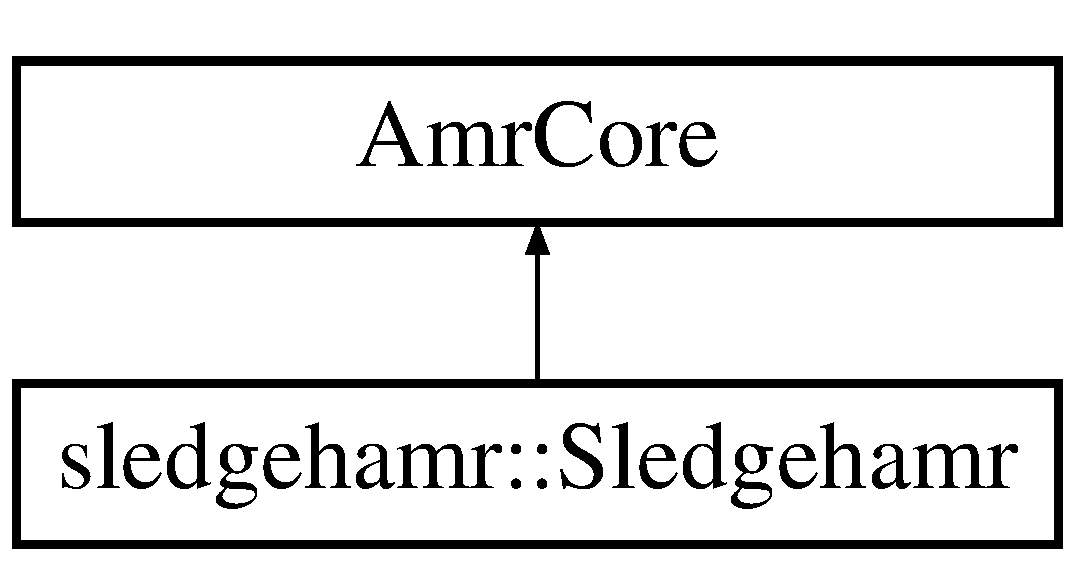
\includegraphics[height=2.000000cm]{classsledgehamr_1_1Sledgehamr}
\end{center}
\end{figure}
\subsection*{Public Member Functions}
\begin{DoxyCompactItemize}
\item 
\mbox{\Hypertarget{classsledgehamr_1_1Sledgehamr_aa79a7ecd89061020a65f5259a286bc3a}\label{classsledgehamr_1_1Sledgehamr_aa79a7ecd89061020a65f5259a286bc3a}} 
\mbox{\hyperlink{classsledgehamr_1_1Sledgehamr_aa79a7ecd89061020a65f5259a286bc3a}{Sledgehamr}} ()
\begin{DoxyCompactList}\small\item\em Creates instances of submodules and reads input parameters. \end{DoxyCompactList}\item 
\mbox{\Hypertarget{classsledgehamr_1_1Sledgehamr_ac68165a48b6802a8910c19c89524975d}\label{classsledgehamr_1_1Sledgehamr_ac68165a48b6802a8910c19c89524975d}} 
void \mbox{\hyperlink{classsledgehamr_1_1Sledgehamr_ac68165a48b6802a8910c19c89524975d}{Init\+Sledgehamr}} ()
\begin{DoxyCompactList}\small\item\em Initalizes data from scratch or from checkpoint file. \end{DoxyCompactList}\item 
\mbox{\Hypertarget{classsledgehamr_1_1Sledgehamr_a356dc1022d4a792e67ee5af0bab4854c}\label{classsledgehamr_1_1Sledgehamr_a356dc1022d4a792e67ee5af0bab4854c}} 
void \mbox{\hyperlink{classsledgehamr_1_1Sledgehamr_a356dc1022d4a792e67ee5af0bab4854c}{Evolve}} ()
\begin{DoxyCompactList}\small\item\em Starts the evolution. \end{DoxyCompactList}\item 
virtual void \mbox{\hyperlink{classsledgehamr_1_1Sledgehamr_acf3cdcc305af82ca3ce9efa61c9fc318}{Fill\+Rhs}} (amrex\+::\+Multi\+Fab \&rhs\+\_\+mf, const amrex\+::\+Multi\+Fab \&state\+\_\+mf, const double time, const int lev, const double \mbox{\hyperlink{classsledgehamr_1_1Sledgehamr_a9239f0c77e572cc155e33f602c19b8dc}{dt}}, const double dx)=0
\begin{DoxyCompactList}\small\item\em Virtual function that loops over a state to fill the R\+HS. Has to be defined by derived project class, though this will be hidden from the user. Reason for this is so that the R\+HS function, declared also by the project class, can be inlined within this function, which it otherwise couldn\textquotesingle{}t as it is not clear at compile time which project will be run. \end{DoxyCompactList}\item 
virtual void \mbox{\hyperlink{classsledgehamr_1_1Sledgehamr_a61bd3ef11742f97b3588aded1c21a688}{Fill\+Add\+Rhs}} (amrex\+::\+Multi\+Fab \&rhs\+\_\+mf, const amrex\+::\+Multi\+Fab \&state\+\_\+mf, const double time, const int lev, const double \mbox{\hyperlink{classsledgehamr_1_1Sledgehamr_a9239f0c77e572cc155e33f602c19b8dc}{dt}}, const double dx, const double weight)=0
\begin{DoxyCompactList}\small\item\em Like Fill\+Rhs but the result will be added to rhs\+\_\+mf rather than set. \end{DoxyCompactList}\item 
\mbox{\Hypertarget{classsledgehamr_1_1Sledgehamr_a615719ce6ad99823f3007471a0401eee}\label{classsledgehamr_1_1Sledgehamr_a615719ce6ad99823f3007471a0401eee}} 
double {\bfseries GetL} () const
\item 
double \mbox{\hyperlink{classsledgehamr_1_1Sledgehamr_ae041be553a87d5da3eda5c6dc143c8b8}{Get\+Dx}} (const int lev) const
\item 
\mbox{\Hypertarget{classsledgehamr_1_1Sledgehamr_ad0184437c39c28d57533f127ffb0f58d}\label{classsledgehamr_1_1Sledgehamr_ad0184437c39c28d57533f127ffb0f58d}} 
double {\bfseries Get\+Dt} (const int lev) const
\item 
\mbox{\Hypertarget{classsledgehamr_1_1Sledgehamr_abc83d3b80945e15dcb9e68c4ec38da46}\label{classsledgehamr_1_1Sledgehamr_abc83d3b80945e15dcb9e68c4ec38da46}} 
int {\bfseries Get\+DimN} (const int lev) const
\item 
\mbox{\Hypertarget{classsledgehamr_1_1Sledgehamr_a8233248303597d2e5e9945d5499c6dd6}\label{classsledgehamr_1_1Sledgehamr_a8233248303597d2e5e9945d5499c6dd6}} 
int {\bfseries Get\+Max\+Level} () const
\item 
\mbox{\Hypertarget{classsledgehamr_1_1Sledgehamr_a4f26822420530e092da46245a25f2d84}\label{classsledgehamr_1_1Sledgehamr_a4f26822420530e092da46245a25f2d84}} 
int {\bfseries Get\+Finest\+Level} () const
\item 
\mbox{\Hypertarget{classsledgehamr_1_1Sledgehamr_aa9e307f7e4247731a24ca3dddb60e02c}\label{classsledgehamr_1_1Sledgehamr_aa9e307f7e4247731a24ca3dddb60e02c}} 
amrex\+::\+Vector$<$ amrex\+::\+Geometry $>$ \& {\bfseries Get\+Geometry} ()
\item 
\mbox{\Hypertarget{classsledgehamr_1_1Sledgehamr_ac08726e6e883efe235b9f52d80535b5e}\label{classsledgehamr_1_1Sledgehamr_ac08726e6e883efe235b9f52d80535b5e}} 
\mbox{\hyperlink{classsledgehamr_1_1LevelData}{Level\+Data}} \& {\bfseries Get\+Level\+Data} (const int lev)
\item 
\mbox{\Hypertarget{classsledgehamr_1_1Sledgehamr_ab647eb1ffc9e0c53654b943239ee6c7d}\label{classsledgehamr_1_1Sledgehamr_ab647eb1ffc9e0c53654b943239ee6c7d}} 
\mbox{\hyperlink{classsledgehamr_1_1LevelData}{Level\+Data}} \& {\bfseries Get\+Old\+Level\+Data} (const int lev)
\item 
\mbox{\Hypertarget{classsledgehamr_1_1Sledgehamr_a7350c88f5fbac3293f0d616bd2210084}\label{classsledgehamr_1_1Sledgehamr_a7350c88f5fbac3293f0d616bd2210084}} 
int {\bfseries Get\+Blocking\+Factor} (const int lev) const
\item 
\mbox{\Hypertarget{classsledgehamr_1_1Sledgehamr_aaf7975f1af5492e12a5e0eae9faa53ed}\label{classsledgehamr_1_1Sledgehamr_aaf7975f1af5492e12a5e0eae9faa53ed}} 
std\+::string {\bfseries Get\+Scalar\+Field\+Name} (const int comp) const
\end{DoxyCompactItemize}
\subsection*{Public Attributes}
\begin{DoxyCompactItemize}
\item 
\mbox{\Hypertarget{classsledgehamr_1_1Sledgehamr_a08088a5d33fc94d5aff24ae0facae9d3}\label{classsledgehamr_1_1Sledgehamr_a08088a5d33fc94d5aff24ae0facae9d3}} 
std\+::unique\+\_\+ptr$<$ \mbox{\hyperlink{classsledgehamr_1_1LevelSynchronizer}{Level\+Synchronizer}} $>$ \mbox{\hyperlink{classsledgehamr_1_1Sledgehamr_a08088a5d33fc94d5aff24ae0facae9d3}{level\+\_\+synchronizer}}
\begin{DoxyCompactList}\small\item\em Pointer to synchronization module. \end{DoxyCompactList}\item 
\mbox{\Hypertarget{classsledgehamr_1_1Sledgehamr_af8c1d908670c8e7a86039634003ca9d2}\label{classsledgehamr_1_1Sledgehamr_af8c1d908670c8e7a86039634003ca9d2}} 
std\+::unique\+\_\+ptr$<$ \mbox{\hyperlink{classsledgehamr_1_1IOModule}{I\+O\+Module}} $>$ {\bfseries io\+\_\+module}
\item 
\mbox{\Hypertarget{classsledgehamr_1_1Sledgehamr_a8b820992141c3e1fc4581b39b86fc8a1}\label{classsledgehamr_1_1Sledgehamr_a8b820992141c3e1fc4581b39b86fc8a1}} 
int \mbox{\hyperlink{classsledgehamr_1_1Sledgehamr_a8b820992141c3e1fc4581b39b86fc8a1}{nghost}} = 0
\begin{DoxyCompactList}\small\item\em Number of ghost cells. \end{DoxyCompactList}\item 
\mbox{\Hypertarget{classsledgehamr_1_1Sledgehamr_affbe4047a4e7222e61195b4241ff4bb1}\label{classsledgehamr_1_1Sledgehamr_affbe4047a4e7222e61195b4241ff4bb1}} 
bool {\bfseries with\+\_\+gravitational\+\_\+waves} = false
\item 
\mbox{\Hypertarget{classsledgehamr_1_1Sledgehamr_a6a06d1bf6d7436d39e8f0a809b8293a2}\label{classsledgehamr_1_1Sledgehamr_a6a06d1bf6d7436d39e8f0a809b8293a2}} 
bool {\bfseries do\+\_\+thorough\+\_\+checks} = false
\item 
\mbox{\Hypertarget{classsledgehamr_1_1Sledgehamr_ad2185aafc7053f34e7325584ff808eb3}\label{classsledgehamr_1_1Sledgehamr_ad2185aafc7053f34e7325584ff808eb3}} 
int {\bfseries check\+\_\+mpi\+\_\+ranks} = 0
\item 
\mbox{\Hypertarget{classsledgehamr_1_1Sledgehamr_abec8e744b285c224cc3cba2f23dda06d}\label{classsledgehamr_1_1Sledgehamr_abec8e744b285c224cc3cba2f23dda06d}} 
int {\bfseries nerrors} = 0
\end{DoxyCompactItemize}
\subsection*{Protected Member Functions}
\begin{DoxyCompactItemize}
\item 
virtual void \mbox{\hyperlink{classsledgehamr_1_1Sledgehamr_a29f2cfdb24f159a165d177012ca7f219}{Make\+New\+Level\+From\+Scratch}} (int lev, amrex\+::\+Real time, const amrex\+::\+Box\+Array \&ba, const amrex\+::\+Distribution\+Mapping \&dm) override
\begin{DoxyCompactList}\small\item\em Make a new level from scratch using provided Box\+Array and Distribution\+Mapping. Only used during initialization. Overrides the pure virtual function in amrex\+::\+Amr\+Core. \end{DoxyCompactList}\item 
virtual void \mbox{\hyperlink{classsledgehamr_1_1Sledgehamr_ae6cc40f77442f989b46196439ca1310e}{Make\+New\+Level\+From\+Coarse}} (int lev, amrex\+::\+Real time, const amrex\+::\+Box\+Array \&ba, const amrex\+::\+Distribution\+Mapping \&dm) override
\begin{DoxyCompactList}\small\item\em Make a new level using provided Box\+Array and Distribution\+Mapping, and fills it with interpolated coarse level data. Overrides the pure virtual function in amrex\+::\+Amr\+Core. \end{DoxyCompactList}\item 
virtual void \mbox{\hyperlink{classsledgehamr_1_1Sledgehamr_a66eafb81586abbd98cea7eb7e99db338}{Remake\+Level}} (int lev, amrex\+::\+Real time, const amrex\+::\+Box\+Array \&ba, const amrex\+::\+Distribution\+Mapping \&dm) override
\begin{DoxyCompactList}\small\item\em Remake a new level using provided Box\+Array and Distribution\+Mapping, and fills it with interpolated coarse level data. Overrides the pure virtual function in amrex\+::\+Amr\+Core. \end{DoxyCompactList}\item 
virtual void \mbox{\hyperlink{classsledgehamr_1_1Sledgehamr_a767607bce4ba621f509c6279faa7195f}{Clear\+Level}} (int lev) override
\begin{DoxyCompactList}\small\item\em Delete level data. Overrides the pure virtual function in amrex\+::\+Amr\+Core. \end{DoxyCompactList}\item 
virtual void \mbox{\hyperlink{classsledgehamr_1_1Sledgehamr_ae0a4a4db58d14e9bb4ef38ebc6edadb7}{Error\+Est}} (int lev, amrex\+::\+Tag\+Box\+Array \&tags, amrex\+::\+Real time, int ngrow) override
\begin{DoxyCompactList}\small\item\em Tag cells for refinement. Overrides the pure virtual function in amrex\+::\+Amr\+Core. \end{DoxyCompactList}\item 
virtual void \mbox{\hyperlink{classsledgehamr_1_1Sledgehamr_a14510bc01e24329a95ec7aa2d86ab569}{Tag\+With\+Truncation\+Cpu}} (const amrex\+::\+Array4$<$ const double $>$ \&state\+\_\+fab, const amrex\+::\+Array4$<$ const double $>$ \&state\+\_\+fab\+\_\+te, const amrex\+::\+Array4$<$ char $>$ \&tagarr, const amrex\+::\+Box \&tilebox, double time, int lev, int $\ast$ntags\+\_\+total, int $\ast$ntags\+\_\+user, int $\ast$ntags\+\_\+trunc, const std\+::vector$<$ double $>$ \&params\+\_\+tag, const std\+::vector$<$ double $>$ \&params\+\_\+mod)=0
\begin{DoxyCompactList}\small\item\em Virtual function that loop over a state to tags cells for refinement. Includes user-\/defined tags and truncation error tags. Will automatically be overriden by the project class. \end{DoxyCompactList}\item 
\mbox{\Hypertarget{classsledgehamr_1_1Sledgehamr_af8129bf33797b5d3e64d415e7f9876a5}\label{classsledgehamr_1_1Sledgehamr_af8129bf33797b5d3e64d415e7f9876a5}} 
virtual void {\bfseries Tag\+With\+Truncation\+Gpu} (const amrex\+::\+Array4$<$ const double $>$ \&state\+\_\+fab, const amrex\+::\+Array4$<$ const double $>$ \&state\+\_\+fab\+\_\+te, const amrex\+::\+Array4$<$ char $>$ \&tagarr, const amrex\+::\+Box \&tilebox, double time, int lev, const std\+::vector$<$ double $>$ \&params\+\_\+tag, const std\+::vector$<$ double $>$ \&params\+\_\+mod)=0
\item 
\mbox{\Hypertarget{classsledgehamr_1_1Sledgehamr_a72376b1fc0e22a68c8449bccc6518897}\label{classsledgehamr_1_1Sledgehamr_a72376b1fc0e22a68c8449bccc6518897}} 
virtual void \mbox{\hyperlink{classsledgehamr_1_1Sledgehamr_a72376b1fc0e22a68c8449bccc6518897}{Tag\+Without\+Truncation\+Cpu}} (const amrex\+::\+Array4$<$ const double $>$ \&state\+\_\+fab, const amrex\+::\+Array4$<$ char $>$ \&tagarr, const amrex\+::\+Box \&tilebox, double time, int lev, int $\ast$ntags\+\_\+total, const std\+::vector$<$ double $>$ \&params)=0
\begin{DoxyCompactList}\small\item\em Same as Tag\+With\+Truncation but does not include truncation error tags. \end{DoxyCompactList}\item 
\mbox{\Hypertarget{classsledgehamr_1_1Sledgehamr_acd89d0e95abb1c601a4622c400893c97}\label{classsledgehamr_1_1Sledgehamr_acd89d0e95abb1c601a4622c400893c97}} 
virtual void {\bfseries Tag\+Without\+Truncation\+Gpu} (const amrex\+::\+Array4$<$ const double $>$ \&state\+\_\+fab, const amrex\+::\+Array4$<$ char $>$ \&tagarr, const amrex\+::\+Box \&tilebox, double time, int lev, const std\+::vector$<$ double $>$ \&params)=0
\item 
\mbox{\Hypertarget{classsledgehamr_1_1Sledgehamr_a9c1605a42a34853ce9efb99f7be43a2a}\label{classsledgehamr_1_1Sledgehamr_a9c1605a42a34853ce9efb99f7be43a2a}} 
virtual void \mbox{\hyperlink{classsledgehamr_1_1Sledgehamr_a9c1605a42a34853ce9efb99f7be43a2a}{Init}} ()
\begin{DoxyCompactList}\small\item\em Initialize project specific details. \end{DoxyCompactList}\item 
bool \mbox{\hyperlink{classsledgehamr_1_1Sledgehamr_a55951d4d585f60943a265c02666a38c0}{Do\+Create\+Level\+If}} (const int lev, const double time)
\begin{DoxyCompactList}\small\item\em Function to check whether a given level is allowed to be created by a given time. Can be overridden by the project class. Will always allow a level to be created by default. \end{DoxyCompactList}\item 
\mbox{\Hypertarget{classsledgehamr_1_1Sledgehamr_ac018ba7412bd5e0eebb4be64736aabba}\label{classsledgehamr_1_1Sledgehamr_ac018ba7412bd5e0eebb4be64736aabba}} 
virtual bool {\bfseries Create\+Level\+If} (const int lev, const double time)
\item 
\mbox{\Hypertarget{classsledgehamr_1_1Sledgehamr_a72dbd6348ab3dd777f80f005dada9d56}\label{classsledgehamr_1_1Sledgehamr_a72dbd6348ab3dd777f80f005dada9d56}} 
virtual bool {\bfseries Stop\+Running} (const double time)
\item 
\mbox{\Hypertarget{classsledgehamr_1_1Sledgehamr_a1fc21e49b69617b209794eb3aa7399d9}\label{classsledgehamr_1_1Sledgehamr_a1fc21e49b69617b209794eb3aa7399d9}} 
virtual void {\bfseries Set\+Params\+Rhs} (std\+::vector$<$ double $>$ \&params, const double time, const int lev)
\item 
\mbox{\Hypertarget{classsledgehamr_1_1Sledgehamr_ac17889590166ddca3944bfd28234ee99}\label{classsledgehamr_1_1Sledgehamr_ac17889590166ddca3944bfd28234ee99}} 
virtual void {\bfseries Set\+Params\+Gravitational\+Wave\+Rhs} (std\+::vector$<$ double $>$ \&params, const double time, const int lev)
\item 
\mbox{\Hypertarget{classsledgehamr_1_1Sledgehamr_ad38a472702a9bb491988bdc7ead8f27b}\label{classsledgehamr_1_1Sledgehamr_ad38a472702a9bb491988bdc7ead8f27b}} 
virtual void {\bfseries Set\+Params\+Tag\+Cell\+For\+Refinement} (std\+::vector$<$ double $>$ \&params, const double time, const int lev)
\item 
\mbox{\Hypertarget{classsledgehamr_1_1Sledgehamr_aaf352778e8706f7352bc1909e6bdd2aa}\label{classsledgehamr_1_1Sledgehamr_aaf352778e8706f7352bc1909e6bdd2aa}} 
virtual void {\bfseries Set\+Params\+Truncation\+Modifier} (std\+::vector$<$ double $>$ \&params, const double time, const int lev)
\item 
\mbox{\Hypertarget{classsledgehamr_1_1Sledgehamr_aa19c6b1f0bb4ff23df49baa8c3725d60}\label{classsledgehamr_1_1Sledgehamr_aa19c6b1f0bb4ff23df49baa8c3725d60}} 
virtual void {\bfseries Set\+Params\+Spectra} (std\+::vector$<$ double $>$ \&params, const double time)
\item 
\mbox{\Hypertarget{classsledgehamr_1_1Sledgehamr_ad11ee726fd88f667a6da0a103f42563a}\label{classsledgehamr_1_1Sledgehamr_ad11ee726fd88f667a6da0a103f42563a}} 
virtual void {\bfseries Set\+Params\+Projections} (std\+::vector$<$ double $>$ \&params, const double time)
\item 
\mbox{\Hypertarget{classsledgehamr_1_1Sledgehamr_a203fe3b2f9001a0c5572b3a5d55bbec3}\label{classsledgehamr_1_1Sledgehamr_a203fe3b2f9001a0c5572b3a5d55bbec3}} 
void \mbox{\hyperlink{classsledgehamr_1_1Sledgehamr_a203fe3b2f9001a0c5572b3a5d55bbec3}{Create\+Shadow\+Level}} ()
\begin{DoxyCompactList}\small\item\em Creates a shadow level and evolves it by one time step. Needed to compute truncation errors on the coarse level. \end{DoxyCompactList}\item 
\mbox{\Hypertarget{classsledgehamr_1_1Sledgehamr_a4625543f3cf36f29e1b7daaa05e8c668}\label{classsledgehamr_1_1Sledgehamr_a4625543f3cf36f29e1b7daaa05e8c668}} 
virtual void {\bfseries Before\+Timestep} (const double time)
\end{DoxyCompactItemize}
\subsection*{Protected Attributes}
\begin{DoxyCompactItemize}
\item 
\mbox{\Hypertarget{classsledgehamr_1_1Sledgehamr_aa2e845b6090d41759cc34caa18fe1739}\label{classsledgehamr_1_1Sledgehamr_aa2e845b6090d41759cc34caa18fe1739}} 
std\+::unique\+\_\+ptr$<$ \mbox{\hyperlink{classsledgehamr_1_1TimeStepper}{Time\+Stepper}} $>$ \mbox{\hyperlink{classsledgehamr_1_1Sledgehamr_aa2e845b6090d41759cc34caa18fe1739}{time\+\_\+stepper}}
\begin{DoxyCompactList}\small\item\em Pointer to sub-\/modules. \end{DoxyCompactList}\item 
\mbox{\Hypertarget{classsledgehamr_1_1Sledgehamr_a9aaf5367722a908a86e99393f6fc5aa5}\label{classsledgehamr_1_1Sledgehamr_a9aaf5367722a908a86e99393f6fc5aa5}} 
std\+::unique\+\_\+ptr$<$ \mbox{\hyperlink{classsledgehamr_1_1GravitationalWaves}{Gravitational\+Waves}} $>$ {\bfseries gravitational\+\_\+waves}
\item 
\mbox{\Hypertarget{classsledgehamr_1_1Sledgehamr_a6b6f544d51bc9f4b8e8ca4f4ed58d368}\label{classsledgehamr_1_1Sledgehamr_a6b6f544d51bc9f4b8e8ca4f4ed58d368}} 
std\+::unique\+\_\+ptr$<$ \mbox{\hyperlink{classsledgehamr_1_1PerformanceMonitor}{Performance\+Monitor}} $>$ {\bfseries performance\+\_\+monitor}
\item 
\mbox{\Hypertarget{classsledgehamr_1_1Sledgehamr_ab90902175e4d8af5dc39112b136642be}\label{classsledgehamr_1_1Sledgehamr_ab90902175e4d8af5dc39112b136642be}} 
std\+::vector$<$ \mbox{\hyperlink{classsledgehamr_1_1LevelData}{Level\+Data}} $>$ \mbox{\hyperlink{classsledgehamr_1_1Sledgehamr_ab90902175e4d8af5dc39112b136642be}{grid\+\_\+old}}
\begin{DoxyCompactList}\small\item\em Holds the actual simulation data for all levels at two different states in time. \end{DoxyCompactList}\item 
\mbox{\Hypertarget{classsledgehamr_1_1Sledgehamr_a677eb6121cd9161e9c1ba976d89b694f}\label{classsledgehamr_1_1Sledgehamr_a677eb6121cd9161e9c1ba976d89b694f}} 
std\+::vector$<$ \mbox{\hyperlink{classsledgehamr_1_1LevelData}{Level\+Data}} $>$ {\bfseries grid\+\_\+new}
\item 
\mbox{\Hypertarget{classsledgehamr_1_1Sledgehamr_a0f4b66c05d9b5b7f5f4acb5fc5dfd84b}\label{classsledgehamr_1_1Sledgehamr_a0f4b66c05d9b5b7f5f4acb5fc5dfd84b}} 
bool \mbox{\hyperlink{classsledgehamr_1_1Sledgehamr_a0f4b66c05d9b5b7f5f4acb5fc5dfd84b}{shadow\+\_\+hierarchy}} = false
\begin{DoxyCompactList}\small\item\em Shadow level in case we need it. \end{DoxyCompactList}\item 
\mbox{\Hypertarget{classsledgehamr_1_1Sledgehamr_ada6b4c3b50b154743da391ed7a5be79c}\label{classsledgehamr_1_1Sledgehamr_ada6b4c3b50b154743da391ed7a5be79c}} 
\mbox{\hyperlink{classsledgehamr_1_1LevelData}{Level\+Data}} {\bfseries shadow\+\_\+level}
\item 
\mbox{\Hypertarget{classsledgehamr_1_1Sledgehamr_a9107cfee4ed83f1e8a8478adb5beb496}\label{classsledgehamr_1_1Sledgehamr_a9107cfee4ed83f1e8a8478adb5beb496}} 
\mbox{\hyperlink{classsledgehamr_1_1LevelData}{Level\+Data}} {\bfseries shadow\+\_\+level\+\_\+tmp}
\item 
\mbox{\Hypertarget{classsledgehamr_1_1Sledgehamr_a87fd1439441652a76e34441ac9bc6bde}\label{classsledgehamr_1_1Sledgehamr_a87fd1439441652a76e34441ac9bc6bde}} 
amrex\+::\+Geometry {\bfseries shadow\+\_\+level\+\_\+geom}
\item 
\mbox{\Hypertarget{classsledgehamr_1_1Sledgehamr_adf5dfa6bf28cbd2a7c3acf5928495222}\label{classsledgehamr_1_1Sledgehamr_adf5dfa6bf28cbd2a7c3acf5928495222}} 
std\+::vector$<$ \mbox{\hyperlink{classsledgehamr_1_1ScalarField}{Scalar\+Field}} $\ast$ $>$ \mbox{\hyperlink{classsledgehamr_1_1Sledgehamr_adf5dfa6bf28cbd2a7c3acf5928495222}{scalar\+\_\+fields}}
\begin{DoxyCompactList}\small\item\em Holds pointers to all simulated scalar fields. We assume ownership of all objects within this vector -\/ one day we upgrade to a smart pointer. \end{DoxyCompactList}\item 
\mbox{\Hypertarget{classsledgehamr_1_1Sledgehamr_ab39530956a51008b7eeb2d61f4eb14f5}\label{classsledgehamr_1_1Sledgehamr_ab39530956a51008b7eeb2d61f4eb14f5}} 
double \mbox{\hyperlink{classsledgehamr_1_1Sledgehamr_ab39530956a51008b7eeb2d61f4eb14f5}{t\+\_\+start}}
\begin{DoxyCompactList}\small\item\em Start and end times of the simulation. \end{DoxyCompactList}\item 
\mbox{\Hypertarget{classsledgehamr_1_1Sledgehamr_a307c02ed0980a082fafb88578121df9d}\label{classsledgehamr_1_1Sledgehamr_a307c02ed0980a082fafb88578121df9d}} 
double {\bfseries t\+\_\+end}
\item 
\mbox{\Hypertarget{classsledgehamr_1_1Sledgehamr_a9239f0c77e572cc155e33f602c19b8dc}\label{classsledgehamr_1_1Sledgehamr_a9239f0c77e572cc155e33f602c19b8dc}} 
std\+::vector$<$ double $>$ \mbox{\hyperlink{classsledgehamr_1_1Sledgehamr_a9239f0c77e572cc155e33f602c19b8dc}{dt}}
\begin{DoxyCompactList}\small\item\em Time step size and grid spacing at each level. \end{DoxyCompactList}\item 
\mbox{\Hypertarget{classsledgehamr_1_1Sledgehamr_a50a57ffa146126e84ebe8c3786e7e162}\label{classsledgehamr_1_1Sledgehamr_a50a57ffa146126e84ebe8c3786e7e162}} 
std\+::vector$<$ double $>$ {\bfseries dx}
\item 
\mbox{\Hypertarget{classsledgehamr_1_1Sledgehamr_ae63f7440e3ecaac50023872f8aa23d80}\label{classsledgehamr_1_1Sledgehamr_ae63f7440e3ecaac50023872f8aa23d80}} 
double \mbox{\hyperlink{classsledgehamr_1_1Sledgehamr_ae63f7440e3ecaac50023872f8aa23d80}{cfl}}
\begin{DoxyCompactList}\small\item\em C\+FL criteria. \end{DoxyCompactList}\item 
\mbox{\Hypertarget{classsledgehamr_1_1Sledgehamr_a3b6cac62b23df3148a59a516f4aab93b}\label{classsledgehamr_1_1Sledgehamr_a3b6cac62b23df3148a59a516f4aab93b}} 
double \mbox{\hyperlink{classsledgehamr_1_1Sledgehamr_a3b6cac62b23df3148a59a516f4aab93b}{L}}
\begin{DoxyCompactList}\small\item\em Box length. \end{DoxyCompactList}\item 
\mbox{\Hypertarget{classsledgehamr_1_1Sledgehamr_a7cd2ed06ec7cffa965017fc3858948e3}\label{classsledgehamr_1_1Sledgehamr_a7cd2ed06ec7cffa965017fc3858948e3}} 
std\+::vector$<$ int $>$ \mbox{\hyperlink{classsledgehamr_1_1Sledgehamr_a7cd2ed06ec7cffa965017fc3858948e3}{dimN}}
\begin{DoxyCompactList}\small\item\em Number of cells in each direction for each level. \end{DoxyCompactList}\item 
\mbox{\Hypertarget{classsledgehamr_1_1Sledgehamr_a67d75bdf0fb15f5cfba92a081e694e2b}\label{classsledgehamr_1_1Sledgehamr_a67d75bdf0fb15f5cfba92a081e694e2b}} 
int \mbox{\hyperlink{classsledgehamr_1_1Sledgehamr_a67d75bdf0fb15f5cfba92a081e694e2b}{coarse\+\_\+level\+\_\+grid\+\_\+size}}
\begin{DoxyCompactList}\small\item\em Number of coarse level cells in each direction. \end{DoxyCompactList}\item 
\mbox{\Hypertarget{classsledgehamr_1_1Sledgehamr_a1d32f49c7150d593c48e2952f27f6da9}\label{classsledgehamr_1_1Sledgehamr_a1d32f49c7150d593c48e2952f27f6da9}} 
std\+::vector$<$ double $>$ \mbox{\hyperlink{classsledgehamr_1_1Sledgehamr_a1d32f49c7150d593c48e2952f27f6da9}{te\+\_\+crit}}
\begin{DoxyCompactList}\small\item\em Truncation error thresholds. \end{DoxyCompactList}\item 
\mbox{\Hypertarget{classsledgehamr_1_1Sledgehamr_ab7a2e0686f9fba4e696c0d8988afc853}\label{classsledgehamr_1_1Sledgehamr_ab7a2e0686f9fba4e696c0d8988afc853}} 
std\+::vector$<$ int $>$ \mbox{\hyperlink{classsledgehamr_1_1Sledgehamr_ab7a2e0686f9fba4e696c0d8988afc853}{spectrum\+\_\+ks}}
\begin{DoxyCompactList}\small\item\em T\+O\+DO. \end{DoxyCompactList}\item 
\mbox{\Hypertarget{classsledgehamr_1_1Sledgehamr_a74c116d587474586db4f44ebe5512740}\label{classsledgehamr_1_1Sledgehamr_a74c116d587474586db4f44ebe5512740}} 
std\+::vector$<$ double $>$ {\bfseries dissipation\+\_\+strength}
\item 
\mbox{\Hypertarget{classsledgehamr_1_1Sledgehamr_a355e94b7c7910b4291356530ce2d240a}\label{classsledgehamr_1_1Sledgehamr_a355e94b7c7910b4291356530ce2d240a}} 
bool {\bfseries with\+\_\+dissipation} = false
\item 
\mbox{\Hypertarget{classsledgehamr_1_1Sledgehamr_adccd9747c433c6d79d7393311b58073b}\label{classsledgehamr_1_1Sledgehamr_adccd9747c433c6d79d7393311b58073b}} 
int {\bfseries dissipation\+\_\+order} = 0
\item 
\mbox{\Hypertarget{classsledgehamr_1_1Sledgehamr_ae2c994a4b05f9e29a965d02ab4e1557b}\label{classsledgehamr_1_1Sledgehamr_ae2c994a4b05f9e29a965d02ab4e1557b}} 
bool {\bfseries restart\+\_\+sim} = false
\end{DoxyCompactItemize}
\subsection*{Friends}
\begin{DoxyCompactItemize}
\item 
\mbox{\Hypertarget{classsledgehamr_1_1Sledgehamr_a0ccb1826a0bd0e46961f29854b9bdba2}\label{classsledgehamr_1_1Sledgehamr_a0ccb1826a0bd0e46961f29854b9bdba2}} 
class {\bfseries Level\+Synchronizer}
\item 
\mbox{\Hypertarget{classsledgehamr_1_1Sledgehamr_ad6cb20f04842bddcd2f1169b48a7c124}\label{classsledgehamr_1_1Sledgehamr_ad6cb20f04842bddcd2f1169b48a7c124}} 
class {\bfseries Local\+Regrid}
\item 
\mbox{\Hypertarget{classsledgehamr_1_1Sledgehamr_ae9cfda6f93e5c3d6dc8ae780872aad17}\label{classsledgehamr_1_1Sledgehamr_ae9cfda6f93e5c3d6dc8ae780872aad17}} 
class {\bfseries Time\+Stepper}
\item 
\mbox{\Hypertarget{classsledgehamr_1_1Sledgehamr_ace5bb0fe4232b9b0ced67ff743994e71}\label{classsledgehamr_1_1Sledgehamr_ace5bb0fe4232b9b0ced67ff743994e71}} 
class {\bfseries Integrator}
\item 
\mbox{\Hypertarget{classsledgehamr_1_1Sledgehamr_aefaf6a5e23c7e41338945f20d82a4401}\label{classsledgehamr_1_1Sledgehamr_aefaf6a5e23c7e41338945f20d82a4401}} 
class {\bfseries I\+O\+Module}
\item 
\mbox{\Hypertarget{classsledgehamr_1_1Sledgehamr_a8e87a92be27fc974044d80e742df6879}\label{classsledgehamr_1_1Sledgehamr_a8e87a92be27fc974044d80e742df6879}} 
class {\bfseries Projection}
\item 
\mbox{\Hypertarget{classsledgehamr_1_1Sledgehamr_ac2ea35640432a8a1420bd335b9d2abef}\label{classsledgehamr_1_1Sledgehamr_ac2ea35640432a8a1420bd335b9d2abef}} 
class {\bfseries Spectrum}
\item 
\mbox{\Hypertarget{classsledgehamr_1_1Sledgehamr_ac3267263ae1fe19fb384924d56ee507b}\label{classsledgehamr_1_1Sledgehamr_ac3267263ae1fe19fb384924d56ee507b}} 
class {\bfseries Gravitational\+Waves}
\item 
\mbox{\Hypertarget{classsledgehamr_1_1Sledgehamr_a91368e0e09c8602b0d1df10a13a3fb81}\label{classsledgehamr_1_1Sledgehamr_a91368e0e09c8602b0d1df10a13a3fb81}} 
class {\bfseries Checkpoint}
\item 
\mbox{\Hypertarget{classsledgehamr_1_1Sledgehamr_aa661d765552bf44ea4e4e9878c1ab1ea}\label{classsledgehamr_1_1Sledgehamr_aa661d765552bf44ea4e4e9878c1ab1ea}} 
class {\bfseries Performance\+Monitor}
\end{DoxyCompactItemize}


\subsection{Detailed Description}
Base class for all derived projects. Combines all the ingredients to make this code work. 

\subsection{Member Function Documentation}
\mbox{\Hypertarget{classsledgehamr_1_1Sledgehamr_a767607bce4ba621f509c6279faa7195f}\label{classsledgehamr_1_1Sledgehamr_a767607bce4ba621f509c6279faa7195f}} 
\index{sledgehamr\+::\+Sledgehamr@{sledgehamr\+::\+Sledgehamr}!Clear\+Level@{Clear\+Level}}
\index{Clear\+Level@{Clear\+Level}!sledgehamr\+::\+Sledgehamr@{sledgehamr\+::\+Sledgehamr}}
\subsubsection{\texorpdfstring{Clear\+Level()}{ClearLevel()}}
{\footnotesize\ttfamily void sledgehamr\+::\+Sledgehamr\+::\+Clear\+Level (\begin{DoxyParamCaption}\item[{int}]{lev }\end{DoxyParamCaption})\hspace{0.3cm}{\ttfamily [override]}, {\ttfamily [protected]}, {\ttfamily [virtual]}}



Delete level data. Overrides the pure virtual function in amrex\+::\+Amr\+Core. 


\begin{DoxyParams}{Parameters}
{\em lev} & Level to be deleted. \\
\hline
\end{DoxyParams}
\mbox{\Hypertarget{classsledgehamr_1_1Sledgehamr_a55951d4d585f60943a265c02666a38c0}\label{classsledgehamr_1_1Sledgehamr_a55951d4d585f60943a265c02666a38c0}} 
\index{sledgehamr\+::\+Sledgehamr@{sledgehamr\+::\+Sledgehamr}!Do\+Create\+Level\+If@{Do\+Create\+Level\+If}}
\index{Do\+Create\+Level\+If@{Do\+Create\+Level\+If}!sledgehamr\+::\+Sledgehamr@{sledgehamr\+::\+Sledgehamr}}
\subsubsection{\texorpdfstring{Do\+Create\+Level\+If()}{DoCreateLevelIf()}}
{\footnotesize\ttfamily bool sledgehamr\+::\+Sledgehamr\+::\+Do\+Create\+Level\+If (\begin{DoxyParamCaption}\item[{const int}]{lev,  }\item[{const double}]{time }\end{DoxyParamCaption})\hspace{0.3cm}{\ttfamily [inline]}, {\ttfamily [protected]}}



Function to check whether a given level is allowed to be created by a given time. Can be overridden by the project class. Will always allow a level to be created by default. 


\begin{DoxyParams}{Parameters}
{\em lev} & Level to be created. \\
\hline
{\em time} & Time before which the level would be created. \\
\hline
\end{DoxyParams}
\begin{DoxyReturn}{Returns}
If the given level is allowed to be created. 
\end{DoxyReturn}
\mbox{\Hypertarget{classsledgehamr_1_1Sledgehamr_ae0a4a4db58d14e9bb4ef38ebc6edadb7}\label{classsledgehamr_1_1Sledgehamr_ae0a4a4db58d14e9bb4ef38ebc6edadb7}} 
\index{sledgehamr\+::\+Sledgehamr@{sledgehamr\+::\+Sledgehamr}!Error\+Est@{Error\+Est}}
\index{Error\+Est@{Error\+Est}!sledgehamr\+::\+Sledgehamr@{sledgehamr\+::\+Sledgehamr}}
\subsubsection{\texorpdfstring{Error\+Est()}{ErrorEst()}}
{\footnotesize\ttfamily void sledgehamr\+::\+Sledgehamr\+::\+Error\+Est (\begin{DoxyParamCaption}\item[{int}]{lev,  }\item[{amrex\+::\+Tag\+Box\+Array \&}]{tags,  }\item[{amrex\+::\+Real}]{time,  }\item[{int}]{ngrow }\end{DoxyParamCaption})\hspace{0.3cm}{\ttfamily [override]}, {\ttfamily [protected]}, {\ttfamily [virtual]}}



Tag cells for refinement. Overrides the pure virtual function in amrex\+::\+Amr\+Core. 


\begin{DoxyParams}{Parameters}
{\em lev} & Level on which cells are tagged. \\
\hline
{\em time} & Time of said level. \\
\hline
{\em ngrow} & Grid growth factor. \\
\hline
{\em ntags\+\_\+user} & Counts number of user-\/defined tags. \\
\hline
\end{DoxyParams}
\mbox{\Hypertarget{classsledgehamr_1_1Sledgehamr_a61bd3ef11742f97b3588aded1c21a688}\label{classsledgehamr_1_1Sledgehamr_a61bd3ef11742f97b3588aded1c21a688}} 
\index{sledgehamr\+::\+Sledgehamr@{sledgehamr\+::\+Sledgehamr}!Fill\+Add\+Rhs@{Fill\+Add\+Rhs}}
\index{Fill\+Add\+Rhs@{Fill\+Add\+Rhs}!sledgehamr\+::\+Sledgehamr@{sledgehamr\+::\+Sledgehamr}}
\subsubsection{\texorpdfstring{Fill\+Add\+Rhs()}{FillAddRhs()}}
{\footnotesize\ttfamily virtual void sledgehamr\+::\+Sledgehamr\+::\+Fill\+Add\+Rhs (\begin{DoxyParamCaption}\item[{amrex\+::\+Multi\+Fab \&}]{rhs\+\_\+mf,  }\item[{const amrex\+::\+Multi\+Fab \&}]{state\+\_\+mf,  }\item[{const double}]{time,  }\item[{const int}]{lev,  }\item[{const double}]{dt,  }\item[{const double}]{dx,  }\item[{const double}]{weight }\end{DoxyParamCaption})\hspace{0.3cm}{\ttfamily [pure virtual]}}



Like Fill\+Rhs but the result will be added to rhs\+\_\+mf rather than set. 


\begin{DoxyParams}{Parameters}
{\em rhs\+\_\+mf} & Empty Multi\+Fab to be filled with R\+HS. \\
\hline
{\em state\+\_\+mf} & State from which the R\+HS is to be computed. \\
\hline
{\em time} & Current time. \\
\hline
{\em lev} & Currently level. \\
\hline
{\em dt} & Time step size. \\
\hline
{\em dx} & Grid spacing. \\
\hline
{\em weight} & rhs = weight$\ast$rhs + ... \\
\hline
\end{DoxyParams}
\mbox{\Hypertarget{classsledgehamr_1_1Sledgehamr_acf3cdcc305af82ca3ce9efa61c9fc318}\label{classsledgehamr_1_1Sledgehamr_acf3cdcc305af82ca3ce9efa61c9fc318}} 
\index{sledgehamr\+::\+Sledgehamr@{sledgehamr\+::\+Sledgehamr}!Fill\+Rhs@{Fill\+Rhs}}
\index{Fill\+Rhs@{Fill\+Rhs}!sledgehamr\+::\+Sledgehamr@{sledgehamr\+::\+Sledgehamr}}
\subsubsection{\texorpdfstring{Fill\+Rhs()}{FillRhs()}}
{\footnotesize\ttfamily virtual void sledgehamr\+::\+Sledgehamr\+::\+Fill\+Rhs (\begin{DoxyParamCaption}\item[{amrex\+::\+Multi\+Fab \&}]{rhs\+\_\+mf,  }\item[{const amrex\+::\+Multi\+Fab \&}]{state\+\_\+mf,  }\item[{const double}]{time,  }\item[{const int}]{lev,  }\item[{const double}]{dt,  }\item[{const double}]{dx }\end{DoxyParamCaption})\hspace{0.3cm}{\ttfamily [pure virtual]}}



Virtual function that loops over a state to fill the R\+HS. Has to be defined by derived project class, though this will be hidden from the user. Reason for this is so that the R\+HS function, declared also by the project class, can be inlined within this function, which it otherwise couldn\textquotesingle{}t as it is not clear at compile time which project will be run. 


\begin{DoxyParams}{Parameters}
{\em rhs\+\_\+mf} & Empty Multi\+Fab to be filled with R\+HS. \\
\hline
{\em state\+\_\+mf} & State from which the R\+HS is to be computed. \\
\hline
{\em time} & Current time. \\
\hline
{\em lev} & Currently level. \\
\hline
{\em dt} & Time step size. \\
\hline
{\em dx} & Grid spacing. \\
\hline
\end{DoxyParams}
\mbox{\Hypertarget{classsledgehamr_1_1Sledgehamr_ae041be553a87d5da3eda5c6dc143c8b8}\label{classsledgehamr_1_1Sledgehamr_ae041be553a87d5da3eda5c6dc143c8b8}} 
\index{sledgehamr\+::\+Sledgehamr@{sledgehamr\+::\+Sledgehamr}!Get\+Dx@{Get\+Dx}}
\index{Get\+Dx@{Get\+Dx}!sledgehamr\+::\+Sledgehamr@{sledgehamr\+::\+Sledgehamr}}
\subsubsection{\texorpdfstring{Get\+Dx()}{GetDx()}}
{\footnotesize\ttfamily double sledgehamr\+::\+Sledgehamr\+::\+Get\+Dx (\begin{DoxyParamCaption}\item[{const int}]{lev }\end{DoxyParamCaption}) const\hspace{0.3cm}{\ttfamily [inline]}}

T\+O\+DO\+: Add max lev check and other methods. \mbox{\Hypertarget{classsledgehamr_1_1Sledgehamr_ae6cc40f77442f989b46196439ca1310e}\label{classsledgehamr_1_1Sledgehamr_ae6cc40f77442f989b46196439ca1310e}} 
\index{sledgehamr\+::\+Sledgehamr@{sledgehamr\+::\+Sledgehamr}!Make\+New\+Level\+From\+Coarse@{Make\+New\+Level\+From\+Coarse}}
\index{Make\+New\+Level\+From\+Coarse@{Make\+New\+Level\+From\+Coarse}!sledgehamr\+::\+Sledgehamr@{sledgehamr\+::\+Sledgehamr}}
\subsubsection{\texorpdfstring{Make\+New\+Level\+From\+Coarse()}{MakeNewLevelFromCoarse()}}
{\footnotesize\ttfamily void sledgehamr\+::\+Sledgehamr\+::\+Make\+New\+Level\+From\+Coarse (\begin{DoxyParamCaption}\item[{int}]{lev,  }\item[{amrex\+::\+Real}]{time,  }\item[{const amrex\+::\+Box\+Array \&}]{ba,  }\item[{const amrex\+::\+Distribution\+Mapping \&}]{dm }\end{DoxyParamCaption})\hspace{0.3cm}{\ttfamily [override]}, {\ttfamily [protected]}, {\ttfamily [virtual]}}



Make a new level using provided Box\+Array and Distribution\+Mapping, and fills it with interpolated coarse level data. Overrides the pure virtual function in amrex\+::\+Amr\+Core. 


\begin{DoxyParams}{Parameters}
{\em lev} & Level to be created. \\
\hline
{\em time} & Time of new grid. \\
\hline
{\em ba} & New amrex\+::\+Box\+Array. \\
\hline
{\em dm} & New amrex\+::\+Distribution\+Mapping. \\
\hline
\end{DoxyParams}
\mbox{\Hypertarget{classsledgehamr_1_1Sledgehamr_a29f2cfdb24f159a165d177012ca7f219}\label{classsledgehamr_1_1Sledgehamr_a29f2cfdb24f159a165d177012ca7f219}} 
\index{sledgehamr\+::\+Sledgehamr@{sledgehamr\+::\+Sledgehamr}!Make\+New\+Level\+From\+Scratch@{Make\+New\+Level\+From\+Scratch}}
\index{Make\+New\+Level\+From\+Scratch@{Make\+New\+Level\+From\+Scratch}!sledgehamr\+::\+Sledgehamr@{sledgehamr\+::\+Sledgehamr}}
\subsubsection{\texorpdfstring{Make\+New\+Level\+From\+Scratch()}{MakeNewLevelFromScratch()}}
{\footnotesize\ttfamily void sledgehamr\+::\+Sledgehamr\+::\+Make\+New\+Level\+From\+Scratch (\begin{DoxyParamCaption}\item[{int}]{lev,  }\item[{amrex\+::\+Real}]{time,  }\item[{const amrex\+::\+Box\+Array \&}]{ba,  }\item[{const amrex\+::\+Distribution\+Mapping \&}]{dm }\end{DoxyParamCaption})\hspace{0.3cm}{\ttfamily [override]}, {\ttfamily [protected]}, {\ttfamily [virtual]}}



Make a new level from scratch using provided Box\+Array and Distribution\+Mapping. Only used during initialization. Overrides the pure virtual function in amrex\+::\+Amr\+Core. 


\begin{DoxyParams}{Parameters}
{\em lev} & Level to be created. \\
\hline
{\em time} & Time of new grid. \\
\hline
{\em ba} & New amrex\+::\+Box\+Array. \\
\hline
{\em dm} & New amrex\+::\+Distribution\+Mapping. \\
\hline
\end{DoxyParams}
\mbox{\Hypertarget{classsledgehamr_1_1Sledgehamr_a66eafb81586abbd98cea7eb7e99db338}\label{classsledgehamr_1_1Sledgehamr_a66eafb81586abbd98cea7eb7e99db338}} 
\index{sledgehamr\+::\+Sledgehamr@{sledgehamr\+::\+Sledgehamr}!Remake\+Level@{Remake\+Level}}
\index{Remake\+Level@{Remake\+Level}!sledgehamr\+::\+Sledgehamr@{sledgehamr\+::\+Sledgehamr}}
\subsubsection{\texorpdfstring{Remake\+Level()}{RemakeLevel()}}
{\footnotesize\ttfamily void sledgehamr\+::\+Sledgehamr\+::\+Remake\+Level (\begin{DoxyParamCaption}\item[{int}]{lev,  }\item[{amrex\+::\+Real}]{time,  }\item[{const amrex\+::\+Box\+Array \&}]{ba,  }\item[{const amrex\+::\+Distribution\+Mapping \&}]{dm }\end{DoxyParamCaption})\hspace{0.3cm}{\ttfamily [override]}, {\ttfamily [protected]}, {\ttfamily [virtual]}}



Remake a new level using provided Box\+Array and Distribution\+Mapping, and fills it with interpolated coarse level data. Overrides the pure virtual function in amrex\+::\+Amr\+Core. 


\begin{DoxyParams}{Parameters}
{\em lev} & Level to be remade. \\
\hline
{\em time} & Time of new grid. \\
\hline
{\em ba} & New amrex\+::\+Box\+Array. \\
\hline
{\em dm} & New amrex\+::\+Distribution\+Mapping. \\
\hline
\end{DoxyParams}
\mbox{\Hypertarget{classsledgehamr_1_1Sledgehamr_a14510bc01e24329a95ec7aa2d86ab569}\label{classsledgehamr_1_1Sledgehamr_a14510bc01e24329a95ec7aa2d86ab569}} 
\index{sledgehamr\+::\+Sledgehamr@{sledgehamr\+::\+Sledgehamr}!Tag\+With\+Truncation\+Cpu@{Tag\+With\+Truncation\+Cpu}}
\index{Tag\+With\+Truncation\+Cpu@{Tag\+With\+Truncation\+Cpu}!sledgehamr\+::\+Sledgehamr@{sledgehamr\+::\+Sledgehamr}}
\subsubsection{\texorpdfstring{Tag\+With\+Truncation\+Cpu()}{TagWithTruncationCpu()}}
{\footnotesize\ttfamily virtual void sledgehamr\+::\+Sledgehamr\+::\+Tag\+With\+Truncation\+Cpu (\begin{DoxyParamCaption}\item[{const amrex\+::\+Array4$<$ const double $>$ \&}]{state\+\_\+fab,  }\item[{const amrex\+::\+Array4$<$ const double $>$ \&}]{state\+\_\+fab\+\_\+te,  }\item[{const amrex\+::\+Array4$<$ char $>$ \&}]{tagarr,  }\item[{const amrex\+::\+Box \&}]{tilebox,  }\item[{double}]{time,  }\item[{int}]{lev,  }\item[{int $\ast$}]{ntags\+\_\+total,  }\item[{int $\ast$}]{ntags\+\_\+user,  }\item[{int $\ast$}]{ntags\+\_\+trunc,  }\item[{const std\+::vector$<$ double $>$ \&}]{params\+\_\+tag,  }\item[{const std\+::vector$<$ double $>$ \&}]{params\+\_\+mod }\end{DoxyParamCaption})\hspace{0.3cm}{\ttfamily [protected]}, {\ttfamily [pure virtual]}}



Virtual function that loop over a state to tags cells for refinement. Includes user-\/defined tags and truncation error tags. Will automatically be overriden by the project class. 


\begin{DoxyParams}{Parameters}
{\em state\+\_\+fab} & Data. \\
\hline
{\em state\+\_\+fab\+\_\+te} & Truncation errors. \\
\hline
{\em tagarr} & Tag status. \\
\hline
{\em tilebox} & Current (tile)box. \\
\hline
{\em time} & Current time. \\
\hline
{\em lev} & Current level. \\
\hline
{\em ntags\+\_\+user} & Counts number of user-\/defined tags. \\
\hline
\end{DoxyParams}


The documentation for this class was generated from the following files\+:\begin{DoxyCompactItemize}
\item 
/global/cfs/cdirs/m3166/buschman/sledgehamr/source/sledgehamr.\+h\item 
/global/cfs/cdirs/m3166/buschman/sledgehamr/source/sledgehamr.\+cpp\end{DoxyCompactItemize}

\hypertarget{classsledgehamr_1_1SledgehamrInit}{}\section{sledgehamr\+:\+:Sledgehamr\+Init Class Reference}
\label{classsledgehamr_1_1SledgehamrInit}\index{sledgehamr\+::\+Sledgehamr\+Init@{sledgehamr\+::\+Sledgehamr\+Init}}


Determines with project has been requested. Also feeds extra derived information to amrex\+::\+Amr\+Core.  




{\ttfamily \#include $<$sledgehamr\+\_\+init.\+h$>$}

\subsection*{Public Member Functions}
\begin{DoxyCompactItemize}
\item 
\mbox{\hyperlink{classsledgehamr_1_1Sledgehamr}{Sledgehamr}} $\ast$ \mbox{\hyperlink{classsledgehamr_1_1SledgehamrInit_a177c4d6ec54f960acea4bfde0c8ccd7c}{Create\+Instance}} ()
\begin{DoxyCompactList}\small\item\em Creates instance of requested derived project class. \end{DoxyCompactList}\end{DoxyCompactItemize}


\subsection{Detailed Description}
Determines with project has been requested. Also feeds extra derived information to amrex\+::\+Amr\+Core. 

\subsection{Member Function Documentation}
\mbox{\Hypertarget{classsledgehamr_1_1SledgehamrInit_a177c4d6ec54f960acea4bfde0c8ccd7c}\label{classsledgehamr_1_1SledgehamrInit_a177c4d6ec54f960acea4bfde0c8ccd7c}} 
\index{sledgehamr\+::\+Sledgehamr\+Init@{sledgehamr\+::\+Sledgehamr\+Init}!Create\+Instance@{Create\+Instance}}
\index{Create\+Instance@{Create\+Instance}!sledgehamr\+::\+Sledgehamr\+Init@{sledgehamr\+::\+Sledgehamr\+Init}}
\subsubsection{\texorpdfstring{Create\+Instance()}{CreateInstance()}}
{\footnotesize\ttfamily \mbox{\hyperlink{classsledgehamr_1_1Sledgehamr}{Sledgehamr}} $\ast$ sledgehamr\+::\+Sledgehamr\+Init\+::\+Create\+Instance (\begin{DoxyParamCaption}{ }\end{DoxyParamCaption})}



Creates instance of requested derived project class. 

\begin{DoxyReturn}{Returns}
Pointer to derived class instance cast to base. Returns N\+U\+LL if none found. 
\end{DoxyReturn}


The documentation for this class was generated from the following files\+:\begin{DoxyCompactItemize}
\item 
/global/cfs/cdirs/m3166/buschman/sledgehamr/source/sledgehamr\+\_\+init.\+h\item 
/global/cfs/cdirs/m3166/buschman/sledgehamr/source/sledgehamr\+\_\+init.\+cpp\end{DoxyCompactItemize}

\hypertarget{classsledgehamr_1_1Timer}{}\section{sledgehamr\+:\+:Timer Class Reference}
\label{classsledgehamr_1_1Timer}\index{sledgehamr\+::\+Timer@{sledgehamr\+::\+Timer}}
\subsection*{Public Member Functions}
\begin{DoxyCompactItemize}
\item 
\mbox{\Hypertarget{classsledgehamr_1_1Timer_add5408527073192c7f6384336ba73146}\label{classsledgehamr_1_1Timer_add5408527073192c7f6384336ba73146}} 
{\bfseries Timer} (std\+::string my\+\_\+name)
\item 
\mbox{\Hypertarget{classsledgehamr_1_1Timer_a29cfaea8e9d7669f1b4cfc4cfc8e0fbb}\label{classsledgehamr_1_1Timer_a29cfaea8e9d7669f1b4cfc4cfc8e0fbb}} 
void {\bfseries Start} ()
\item 
\mbox{\Hypertarget{classsledgehamr_1_1Timer_acb5940b4900781df6acaad4cdc42ba6c}\label{classsledgehamr_1_1Timer_acb5940b4900781df6acaad4cdc42ba6c}} 
void {\bfseries Stop} ()
\item 
\mbox{\Hypertarget{classsledgehamr_1_1Timer_a41597a39dce59fe6f58a5639fc69cc5b}\label{classsledgehamr_1_1Timer_a41597a39dce59fe6f58a5639fc69cc5b}} 
double {\bfseries Get\+Total\+Time\+Seconds} ()
\item 
\mbox{\Hypertarget{classsledgehamr_1_1Timer_a25e1c5fa0585a3763b8dbc20be479f0d}\label{classsledgehamr_1_1Timer_a25e1c5fa0585a3763b8dbc20be479f0d}} 
double {\bfseries Get\+Last\+Duration\+Seconds} ()
\item 
\mbox{\Hypertarget{classsledgehamr_1_1Timer_a51bf2fa058461fd28d3c76b286df11e6}\label{classsledgehamr_1_1Timer_a51bf2fa058461fd28d3c76b286df11e6}} 
std\+::string {\bfseries Get\+Name} () const
\item 
\mbox{\Hypertarget{classsledgehamr_1_1Timer_a8aca03d4d3d7b72abb9b5c2c089e9b68}\label{classsledgehamr_1_1Timer_a8aca03d4d3d7b72abb9b5c2c089e9b68}} 
bool {\bfseries Is\+Running} () const
\end{DoxyCompactItemize}


The documentation for this class was generated from the following files\+:\begin{DoxyCompactItemize}
\item 
/global/cfs/cdirs/m3166/buschman/sledgehamr/source/timer.\+h\item 
/global/cfs/cdirs/m3166/buschman/sledgehamr/source/timer.\+cpp\end{DoxyCompactItemize}

\hypertarget{classsledgehamr_1_1TimeStepper}{}\section{sledgehamr\+:\+:Time\+Stepper Class Reference}
\label{classsledgehamr_1_1TimeStepper}\index{sledgehamr\+::\+Time\+Stepper@{sledgehamr\+::\+Time\+Stepper}}


Class that takes care of the sub-\/cycling in time algorithm as well as the scheduling regrids.  




{\ttfamily \#include $<$time\+\_\+stepper.\+h$>$}

\subsection*{Public Member Functions}
\begin{DoxyCompactItemize}
\item 
\mbox{\Hypertarget{classsledgehamr_1_1TimeStepper_a3e07dcb8a5a92cd4a10b8e3e34f5ce57}\label{classsledgehamr_1_1TimeStepper_a3e07dcb8a5a92cd4a10b8e3e34f5ce57}} 
{\bfseries Time\+Stepper} (\mbox{\hyperlink{classsledgehamr_1_1Sledgehamr}{Sledgehamr}} $\ast$owner)
\item 
void \mbox{\hyperlink{classsledgehamr_1_1TimeStepper_a029f92dcddadc58f020a528cd93da35d}{Advance}} (int lev)
\begin{DoxyCompactList}\small\item\em Recursive function and the core of the sub-\/cycling in time algorithm. Advances a given level by dt\mbox{[}level\mbox{]}. \end{DoxyCompactList}\end{DoxyCompactItemize}
\subsection*{Public Attributes}
\begin{DoxyCompactItemize}
\item 
\mbox{\Hypertarget{classsledgehamr_1_1TimeStepper_a5bf9f74cdd6c280390417bf5c202b824}\label{classsledgehamr_1_1TimeStepper_a5bf9f74cdd6c280390417bf5c202b824}} 
std\+::vector$<$ double $>$ \mbox{\hyperlink{classsledgehamr_1_1TimeStepper_a5bf9f74cdd6c280390417bf5c202b824}{regrid\+\_\+dt}}
\begin{DoxyCompactList}\small\item\em Vector of regridding intervals at each level. \end{DoxyCompactList}\item 
\mbox{\Hypertarget{classsledgehamr_1_1TimeStepper_ad6770cb1fe15aac86e1d3177871e3a59}\label{classsledgehamr_1_1TimeStepper_ad6770cb1fe15aac86e1d3177871e3a59}} 
std\+::unique\+\_\+ptr$<$ Integrator $>$ \mbox{\hyperlink{classsledgehamr_1_1TimeStepper_ad6770cb1fe15aac86e1d3177871e3a59}{integrator}}
\begin{DoxyCompactList}\small\item\em Pointer to integration module. \end{DoxyCompactList}\item 
\mbox{\Hypertarget{classsledgehamr_1_1TimeStepper_a72c737467fbb1dd826d088256708d652}\label{classsledgehamr_1_1TimeStepper_a72c737467fbb1dd826d088256708d652}} 
std\+::unique\+\_\+ptr$<$ Local\+Regrid $>$ {\bfseries local\+\_\+regrid}
\item 
\mbox{\Hypertarget{classsledgehamr_1_1TimeStepper_aa8f91c75fad99d45941504c7694198a8}\label{classsledgehamr_1_1TimeStepper_aa8f91c75fad99d45941504c7694198a8}} 
std\+::unique\+\_\+ptr$<$ \mbox{\hyperlink{classsledgehamr_1_1RegridScheduler}{Regrid\+Scheduler}} $>$ {\bfseries scheduler}
\end{DoxyCompactItemize}


\subsection{Detailed Description}
Class that takes care of the sub-\/cycling in time algorithm as well as the scheduling regrids. 

\subsection{Member Function Documentation}
\mbox{\Hypertarget{classsledgehamr_1_1TimeStepper_a029f92dcddadc58f020a528cd93da35d}\label{classsledgehamr_1_1TimeStepper_a029f92dcddadc58f020a528cd93da35d}} 
\index{sledgehamr\+::\+Time\+Stepper@{sledgehamr\+::\+Time\+Stepper}!Advance@{Advance}}
\index{Advance@{Advance}!sledgehamr\+::\+Time\+Stepper@{sledgehamr\+::\+Time\+Stepper}}
\subsubsection{\texorpdfstring{Advance()}{Advance()}}
{\footnotesize\ttfamily void sledgehamr\+::\+Time\+Stepper\+::\+Advance (\begin{DoxyParamCaption}\item[{int}]{lev }\end{DoxyParamCaption})}



Recursive function and the core of the sub-\/cycling in time algorithm. Advances a given level by dt\mbox{[}level\mbox{]}. 


\begin{DoxyParams}{Parameters}
{\em lev} & Level to be advanced. \\
\hline
\end{DoxyParams}


The documentation for this class was generated from the following files\+:\begin{DoxyCompactItemize}
\item 
/global/cfs/cdirs/m3166/buschman/sledgehamr/source/time\+\_\+stepper.\+h\item 
/global/cfs/cdirs/m3166/buschman/sledgehamr/source/time\+\_\+stepper.\+cpp\end{DoxyCompactItemize}

%--- End generated contents ---

% Index
\backmatter
\newpage
\phantomsection
\clearemptydoublepage
\addcontentsline{toc}{chapter}{Index}
\printindex

\end{document}
